\documentclass[areasetadvanced]{scrartcl}

\usepackage[utf8]{inputenc}
\usepackage[T2A]{fontenc}
\usepackage[english,russian]{babel}

\usepackage[footskip=1cm,left=25mm, right=15mm, top=20mm, bottom=20mm]{geometry}
\usepackage{setspace}
\usepackage{amsmath, amssymb} 
\usepackage{graphicx}
\usepackage{tikz}
\usetikzlibrary{arrows.meta}
\usepackage{float}
\usepackage{dashrule}
\usepackage{fancyhdr} 
\usepackage{hyperref} 
\usepackage{parskip}
\usepackage{textcomp, enumitem}
\usepackage{indentfirst}
\usepackage{graphicx}
\usepackage{algorithm}
\usepackage{algpseudocode}
\usepackage{array} 
\usepackage{geometry}
\usepackage{afterpage}
\usepackage{minted}
\setcounter{secnumdepth}{3} 
\setcounter{tocdepth}{3}    
\usepackage{listings}
\usepackage{xcolor}
\usepackage{caption}
\captionsetup[table]{justification=raggedleft,singlelinecheck=off}

\newcommand{\icon}[1]{\includegraphics[height=1.2em]{\#1}}

\tikzstyle{block} = [rectangle, rounded corners, minimum width=3cm, minimum height=1cm, text centered, draw=black, fill=lightgray]

\setkomafont{sectioning}{\normalfont\bfseries} 
\setkomafont{section}{\normalfont\Large\bfseries}
\setkomafont{subsection}{\normalfont\large\bfseries}
\setkomafont{subsubsection}{\normalfont\large\bfseries}
\setkomafont{paragraph}{\normalfont\large\bfseries} 

\lstset{
  language=Haskell,
  basicstyle=\ttfamily\small,
  keywordstyle=\color{blue}\bfseries,
  stringstyle=\color{red},
  commentstyle=\color{green!70!black},
  numbers=left,
  numberstyle=\tiny,
  stepnumber=1,
  numbersep=10pt,
  showstringspaces=false,
  breaklines=true,
  frame=single
}

\lstdefinelanguage{Lua}{
    keywords={function, end, if, then, else, elseif, for, while, do, repeat, until, break, return, local, and, or, not, true, false, nil},
    keywordstyle=\color{blue}\bfseries,
    stringstyle=\color{red},
    commentstyle=\color{green!70!black},
    morestring=[s]{"}{"},
    morestring=[s]{'}{'},
    morecomment=[l]{ -},
    morecomment=[s]{ -[[}{]]},
    basicstyle=\ttfamily\small,
    numbers=left,
    numberstyle=\tiny,
    stepnumber=1,
    numbersep=10pt,
    showstringspaces=false,
    breaklines=true,
    frame=single
}

\setlength{\parindent}{1.25cm}
\setcounter{tocdepth}{3}
\begin{document}
\sloppy
	\thispagestyle{empty}
	\begin{center}
		\large{МИНОБРНАУКИ РОССИИ} \par
		\vspace{0.3cm}
		\normalsize
		{ФЕДЕРАЛЬНОЕ ГОСУДАРСТВЕННОЕ АВТОНОМНОЕ ОБРАЗОВАТЕЛЬНОЕ УЧРЕЖДЕНИЕ ВЫСШЕГО ОБРАЗОВАНИЯ} \par
		\vspace{0.3cm}
		\textbf{\guillemotleft САНКТ-ПЕТЕРБУРГСКИЙ ПОЛИТЕХНИЧЕСКИЙ}
		\textbf{УНИВЕРСИТЕТ ПЕТРА ВЕЛИКОГО\guillemotright} \par
		\vspace{0.3cm}
		{Институт компьютерных наук и кибербезопасности}\par
        \vspace{0.3cm}
    \end{center}
    \noindent
    \setlength{\tabcolsep}{0.6em}
    \renewcommand{\arraystretch}{1.35}
    \begin{tabular}{@{}p{0.32\textwidth}@{\hspace{1cm}}p{0.12\textwidth}@{\hspace{1cm}}p{0.38\textwidth}@{}}
        Направление подготовки & 02.03.01 & Математика и компьютерные науки \\[0.6em]
        Направленность подготовки бакалавриата & 02.03.01\_01 & Системы искусственного интеллекта и суперкомпьютерные технологии \\[0.7em]
        Квалификация & & Бакалавр \\[0.6em]
        Институт & & Компьютерных наук и кибербезопасности \\[0.6em]
        Кафедра & & Высшая школа технологий искусственного интеллекта \\[0.6em]
        Дисциплина & & Генетические алгоритмы \\[0.6em]
        Курс & 4 & Группа 5130201/20101
    \end{tabular}
        \vspace{1.5cm}
        \begin{center}        
        \par
        
        { \textbf{ПОИСК ГИПЕРПАРАМЕТРОВ И ВЫБОР МОДЕЛИ СЕГМЕНТАТОРА ДЛЯ ЗАДАЧИ ВЫДЕЛЕНИЯ ЗОНЫ ИНТЕРЕСА ТРАМВАЙНЫХ ПУТЕЙ}}\par
        
        \textbf{}\par
        
        \end{center}
        \vfill
        \begin{flushleft}
        
        Студент: \hspace{1.8cm} \rule[0pt]{2.5cm}{0.5pt}\hfill Салимли Айзек Мухтар Оглы\par
        
        \vspace{0.5cm}
        
        Преподаватель: \hspace{0.55cm} \rule[0pt]{2.5cm}{0.5pt}\hfill Большаков Александр Афанасьевич
        
        \end{flushleft}
        
        \vspace{0.5cm}
        
        \begin{flushright}
        
        \guillemotleft \rule[0pt]{0.8cm}{0.5pt}\guillemotright \rule[0pt]{2cm}{0.5pt} 20\rule[0pt]{0.5cm}{0.5pt} г.
        
        \end{flushright}
        
        \vfill
        
        \begin{center}
        
        Санкт-Петербург, 2026
        
        \end{center}

\newpage
\par\noindent
{\centering
\usekomafont{section}ЗАДАНИЕ\par
\vspace{1.5ex}
}
\noindent
\begin{enumerate}[label=\arabic*., ref=\arabic*]
    \item Тема работы: \guillemotleft Распознование посторонних объектов на трамвайных рельсах в режиме реального времени.\guillemotright
    \begin{enumerate}[label=\arabic{enumi}.\arabic*., ref=\arabic{enumi}.\arabic*]
        \item Скобцов, Ю. А. Эволюционные вычисления: Учебное пособие / Ю. А. Скобцов, Д. В. Сперанский. – М.: Национальный Открытый Университет «ИНТУИТ», 2012. – 331с., ил. – (Серия «Основы информационных технологий»).
        \item Алиев М. В., Бербенцев Д. А., Немыкин В. О., Алиева С. М. Алгоритмы распознавания объектов в видеопотоке и определение свойств их взаимного расположения // Вестник Адыгейского государственного университета. Сер. Естественно-математические и технические науки. – 2024. – № 2(341). – С. 27–34. DOI: 10.53598/2410-3225-2024-2-341-27-34.
        \item Зотов С. С., Яковлев А. А., Колчищев Д. А. Обнаружение объектов в реальном времени с помощью алгоритмов распознавания YOLO // Синергия наук. – 2018. – № 23. – С. 1245–1261.
        \item Чочиа П. А. Сегментация изображений на основе анализа расстояний в пространстве признаков // Информационные процессы. - 2020. - № 6. - С. 97-110.
        \item Zhang H., Ullah N, Sharnah A. CA-SegFormer: An improved coordinate attention-enchanced model for crack segmentation in concrete structures // Case Studies in Construction Materials. - 2025. - Vol. 23.
        \item Yanyan Z., Zhiliang S. Adioc loss: An Auxiliary descent IoC loss function // Engineering Applications of Artificial Intelligence - 2022. - №105453. - с. 117-133. DOI: https://doi.org/10.1016/j.engappai.2022.105453.
        \item YOLOv8 Documentation [Электронный ресурс] // Ultralytics. - Доступ: https://docs.ultralytics.com/ru/models/yolov8/ (Дата обращения: 07.02.2026).
        \item YOLOv5 Documentation [Электронный ресурс] // Ultralytics. - Доступ: https://docs.ultralytics.com/ru/models/yolov5/ (Дата обращения: 07.02.2026).
        \item Xie E., Wang W., Yu Z., Anandkumar A., Alvarez J. M., Luo P. SegFormer: Simple and Efficient Design for Semantic Segmentation with Transformers // arXiv [cs.CV]. – 2021. – 28 Oct.
        \item RailSafeNet. train\_SegFormer.py [Электронный ресурс] // GitHub. – Доступ: https://github.com/oValach/RailSafeNet/blob/main/train\_SegFormer.py (Дата обращения: 14.03.2026).
        \item Мороз Е. С., Пикалёв Я. С. Анализ SOTA-архитектур для семантической аугментации // Информационные технологии и системы. – 2025. – № 4. – С. 39–60. DOI: 10.24412/2413-7383-2025-4-39-60-70.
        \item Xie E., Wang W., Yu Z., Anandkumar A., Alvarez J. M., Luo P. Details of MiT Series // arXiv [cs.CV]. – 2021. – (Supplementary material).
        \item DeepLabV3Plus-RailSem19 [Электронный ресурс] // GitHub. – Доступ: https://github.com/pideyi1025/DeepLabV3Plus-RailSem19/tree/main (Дата обращения: 14.03.2026).
        \item Springer Link. Статья по компьютерному зрению [Электронный ресурс] // Springer. – Доступ: https://link.springer.com/article/10.1007/s11554-023-01380-x (Дата обращения: 14.03.2026).
        \item Instance Segmentation. Val [Электронный ресурс] // Ultralytics. – Доступ: https://docs.ultralytics.com/ru/tasks/segment/\#val (Дата обращения: 14.03.2026).
        \item YOLOv8. Key Features [Электронный ресурс] // Ultralytics. – Доступ: https://docs.ultralytics.com/ru/models/yolov8/\#key-features-of-yolov8 (Дата обращения: 14.03.2026).
        \item YOLOv11. Key Features [Электронный ресурс] // Ultralytics. – Доступ: https://docs.ultralytics.com/ru/models/yolov11/\#key-features-of-yolov11 (Дата обращения: 14.03.2026).
        \item YOLO26 Documentation [Электронный ресурс] // Ultralytics. – Доступ: https://docs.ultralytics.com/ru/models/yolo26/ (Дата обращения: 14.03.2026).
        \item Hyperparameter Tuning [Электронный ресурс] // Ultralytics. – Доступ: https://docs.ultralytics.com/guides/hyperparameter-tuning/ (Дата обращения: 14.03.2026).
    \end{enumerate}
    \item Содержание работы
    \begin{enumerate}[label=\arabic{enumi}.\arabic*., ref=\arabic{enumi}.\arabic*]
        \item Введение
        \item Актуальность темы
        \item Постановка задачи
        \item Компьютерное зрение и задача сегментации
        \item Сегментатор SegFormer
        \item Сегментатор DeepLabV3+ ResNet101
        \item Сегментатор YOLO-seg
        \item Подбор гиперпараметров методом эволюционной стратегии
        \item Выбор метода минимизации функции потерь
        \item Обучение сегментатора
        \item Анализ результатов
        \item Заключение
    \end{enumerate}
    \item Дата выдачи задания \guillemotleft 6\guillemotright февраля 2026 г.
\end{enumerate}

Преподаватель: \hspace{0.55cm} \rule[0pt]{2.5cm}{0.5pt}\hfill Большаков А.А.

Задание принято к исполнению \guillemotleft 6\guillemotright февраля 2026 г.

Студент: \hspace{0.55cm} \rule[0pt]{2.5cm}{0.5pt}\hfill Салимли А.М.


\newpage
\tableofcontents

\newpage
\section*{Введение}
\addcontentsline{toc}{section}{Введение}

Обнаружение посторонних объектов на трамвайных путях - практическая задача для систем компьютерного зрения. В данной работе предлагается следующий подход: на первом этапе передачи видеопотока выполняется сегментация рельсов с помощью исследуемых моделей (SegFormer, DeepLabV3+ ResNet101, YOLOv8n-seg, YOLOv8s-seg, YOLOv11s-seg, YOLO26s-seg); на втором этапе с помощью библиотеки opencv дорисовываются ограничения опасной зоны котороя является зоной рельс и прилегающей к ним области по ширине трамвая; далее на третьем этапе в выделенной опасной зоне применяется детектор YOLOv8 в режиме инференса для распознавания посторонних объектов в реальном времени (\textbf{\textcolor{red}{второй и третий этапы не входит в курсовую работу}}).

Обучается не модель детекции (YOLOv8 используется только на этапе инференса), а сегментатор. Для выбора модели сегментатора, расматриваются три модели с разными архитектурами, в последствие сравнения, выбирается сегментатор удовлетваряющий критериям реального времени $30 FPS$ и точности не менее $70\%$. Для таких задач требуется правильный подбор гиперпараметров и оптимизация функции потерь сегментатора. Стандартным промышленным подходом для минимизации функции потерь являются методы градиентного спуска, в частности стохастический градиентный спуск (SGD) и его адаптивные варианты. В рамках данной курсовой работы рассматривается генетический алгоритм основанный на эволюционной стратегии, для обеспечения автоматического подбора гиперпараметров и выбор алгоритма минимизации функции потерь сегментатора с помощью генетических алгоритмов и методов градиентного спуска.

Результатом работы является вывод оптимальных гиперпараметров для обучения сегментатора, выбор модели сегментатора и алгоритм минимизации функции потерь сегментатора.

В качестве генетических алгоритмов для минимизации функции потерь рассматриваются:
\begin{itemize}
    \item Эволюционная стратегия с ковариационной матрицей из библиотеки \textbf{torch} (CMA-ES);
\end{itemize}

В качестве градиентных методов для минимизации функции потерь рассматриваются:
\begin{itemize}
    \item Стохастический градиентный спуск (SGD);
    \item Адаптивный метод с разделением затухания весов из библиотеки \textbf{torch} (AdamW).
\end{itemize}

Для подбора гиперпараметров используется метод эволюционной стратегии, работающий по принципу отбора лучших особей (наборов гиперпараметров) по целевой метрике (fitness) и генерации новых кандидатов путём мутации.

В библиотеке Ultralytics метод \texttt{tune()} реализует подбор гиперпараметров на основе генетического алгоритма: задаётся начальный набор гиперпараметров и допустимая область поиска; на каждой итерации к текущему набору применяется оператор мутации (\texttt{\_mutate}), получаемые варианты используются для обучения модели, после чего по метрикам (AP50, F1-score и др.) вычисляется fitness; в следующих итерациях эволюция опирается на наиболее успешные конфигурации. Кроссовер в базовой реализации не используется - поиск ведётся преимущественно за счёт мутации. Процесс повторяется до достижения заданного числа итераций или требуемого качества; результаты сохраняются (в том числе в CSV), оптимальные гиперпараметры выводятся в отдельный файл.

\newpage
\section{Актуальность темы}
Планируемое открытие новых высокоскоростных трамвайных линий в Санкт-Петербурге повышает требования к надежности и скорости реакции систем мониторинга.
Существующие методы визуального контроля, основанные на наблюдении персонала, иногда не обеспечивают необходимой полноты, непрерывности и быстродействия,  
особенно в условиях интенсивного городского трафика, плохой видимости или сложной погодной обстановки.

Следовательно, создание автоматизированной системы, способной в режиме реального времени с высокой точностью детектировать посторонние объекты на путях, 
является актуальной научно-прикладной задачей. Ее решение должно позволить, минимизировать риски аварийных ситуаций и повысить 
общую надежность и безопасность работы городского электротранспорта. Данное исследование посвящено сравнительному анализу методов оптимизации для минимизации функции потерь (градиентный спуск и генетические алгоритмы), выбор метода подбора гиперпараметров (генетический алгоритм) и конечный выбор модели сегментатора и направлено на поиск наиболее эффективного технического решения.

Такая система, может служить как вспомогательная система для водителя трамвая или основой для создания системы беспилотных трамваев.

\newpage
\section{Постановка задачи}
В данной курсовой работе необходимо:
\begin{enumerate}
    \item Найти или подготовить размеченный датасет изображений трамвайных путей;
    \item Сформировать критерий реального времени для полного прогона конвеера (сегментация кадра, дорисовка опасной зоны, детекция объектов);
    \item Разбить датасет на части обучения, валидации и тестирования;
    \item Изучить скорости и точность инференса сегментаторов;
    \item На основе стандартного обучения сегментатора, выбрать оптимальную модель;
    \item Реализовать подбор гиперпараметров методом эволюционной стратегии;
    \item Выбрать метод минимизации функции потерь;
    \item Обучить сегментатор на выбранной модели и методе минимизации функции потерь;
    \item Провести анализ результатов.
\end{enumerate}

\newpage
\section{Компьютерное зрение и задача сегментации}
Компьютерное зрение (Computer Vision) - это научная область искусственного интеллекта, целью которой является создание моделей и алгоритмов для автоматического извлечения,
анализа и понимания полезной информации из цифровых изображений или видеопотоков. Формально, это задача преобразования данных из исходного пространства высокомерных пикселей
(матрицы интенсивностей), в компактное пространство семантических описаний, пригодных для
принятия решений. Формально можно задать отображение:

$$
    I(h,w) \rightarrow T_r,
$$

где $h$ - высота изображения, $w$ - ширина изображения, а $T_r$ это пространство семантических описаний, пригодных для принятий решения. 

В случае поставленной задачи, $T_r$ - будет являтся разделенное изображение на семантически значемые области или экземпляры объектов.

Описаная задача, называется сегментацией изображения. 

Подход сегментации можно рассматреть как разбиение изображения на однородные области на основе анализа расстояний в пространстве признаков.

Можно более точно задать теоретико-множественную модель как отображение множества точек изображения в конечный набор значений (меток сегментов):

$$
    F : Img \rightarrow {1,2, \dots Q},
$$
где Q - итоговое число сегментов. Критерием однородности служит оценка близости точек в объедененном пространстве признаков.

Пространство можно описать так:

Множество точек изображения $I(h,w)$, на дискретной решетке:
$$  
    \Omega = {(h,w) | h = 1, \dots, H, w = 1, \dots, W}
$$

Каждой точке, сопоставлен вектор интенсивности RGB:

$$
    x(h,w) \in \mathbb{R}^3
$$

Тогда исходное пространство:

$$
    I_s = {x(h,w) | ((h,w) \in I)}\subset \mathbb{R}^3
$$

Помимо цвета RGB, точке может быть присвоены инные признаки (в SegFormer эти признаки делятся на 4 уровня), например - контекстовый эмбеддинг вектора, семантические признаки.

Это пространство признаков $F \subset \mathbb{R}^d$

Тогда получаем отображение множества исходного пространство в множество пространства признаков. 

$$
    Prepare : I_s \rightarrow F
$$

То есть для каждого пикселя получая вектор признаков:

$$
    \vec{v}(h,w) = Prepare(x(h,w)) \in \mathbb{R}^d
$$

За отображение точек в признаки, отвечает Encoder, после того как признаки были присвоены всем пикселям в изображение,
они поступают на вход в Decoder, который отвечает за классификацию через слои нейронной сети получая на выходе тензоры, проходящие через $Argmax$, в результате чего идет преобразование тензора в пиксель. Далее к каждому декодированному пикселю применяется функция $Softmax$, которая 
присваивает вероятности принадлежности пикселя к классу и дорисовывается маска сегментации.

\newpage
\section{Сегментатор SegFormer}
Сегментация формулируется как задача попиксельной классификации, решаемая нейронной сетью.

Математически такая сегментация описывается как присвоение каждому пикселю входного изображения метки класса.
SegFormer - представляет собой структуру энкодер-декодера работающий по следующему алгоритму:

\begin{itemize}
    \item Иерархический трансформер-энкодер: \begin{itemize}
            \item Входное изображение $H \times W \times 3$ разбивается на батчи
            \item Энкодер генерирует многоуровневые признаки $F_i$, с разрешением $\frac{H}{4}, \frac{H}{8}, \frac{H}{16}, \frac{H}{32}$
            \item Далее механизм внимания, который снижает вычислительную сложность за счет уменьшения размерностей ключей $K$:
                $$ Attention(Q,K,V) = Softmax(\frac{QK^T}{\sqrt{d_{head}}}) V $$
                $$ \hat{K} = Reshape{K}, K = Linear(\hat{K}) $$
        \end{itemize}
    \item Координатное внимание: \begin{itemize}
        \item Координатное внимание кодирует входное изображение по вертикали $z_{n}^{h}$ и по горизонтали $z_{n}^{w}$
        \item Далее кодируются точки по диагонали по главной $z_{n}^{m}$ и второстепенной $z_{n}^{v}$
                $$ z_{n}^{h}(h) = \frac{1}{W} \sum_{i = 0}^{\min{H,W}} x_n(h,i) $$
                $$ z_{n}^{w}(w) = \frac{1}{H} \sum_{j = 0}^{\min{H,W}} x_n(j,w) $$
                $$ z_{n}^{m}(k) = \frac{1}{\min{H,W}} \sum_{k = 0}^{\min{H,W}} x_n(k,k) $$
                $$ z_{n}^{v}(l) = \frac{1}{\min{H,W}} \sum_{l = 0}^{\min{H,W}} x_n(l, H - 1 - l) $$ 
        \item Эти карты признаков конкатинируются и обрабатываются свертками $1 \times 1$, для получения тензора внимания $f$, который затем разделяется обратно на 4 направления.
        \item Финальные веса $g$ применяются к исходным признакам:
                $$ y_n(i, j) = x_n(i,j) \cdot g_n^h(i) \cdot g_n^w(j) \cdot g_n^m(k) \cdot g_n^v(l) $$
    \end{itemize}
    \item После кодирования применяется легковесный MLP-декодер: \begin{itemize}
        \item Признаки $F_i$ от энкодера нормализуются и приводятся к единой размерности каналов $C$: $\hat{F_i} = Linear(C_i, C)(F_i) $
        \item Все $\hat{F_i}$ апсемплятся до разрешения $\frac{H}{4} \times \frac{W}{4}$
        \item После признаки конкатенируются и пропускаются через MLP-слой для слияния: 
            $$ F = Linear(4C,C)(Concat(\hat{F_i})) $$
        \item Финальный слой MLP предсказывает маску сегментации $M$ размерности $\frac{H}{4} \times \frac{W}{4} \times N_{cls}$, где $N_{cls}$ - число классов.
    \end{itemize}
\end{itemize}

Для оценки качества сегментации используются метрики Precision и Recall которые вычисляются на основе пикселей матрицы ошибок (TP, FP, TN, FN).

Precision - отвечает за то, сколько доля правильных объектов среди всех, посчитала нейросеть.

Recall - отвечает за то, сколько всего найденных объектов среди всех реальных на картинке. 

Целевой функцией для минимизации, является функция потерь Sparse Crosss-Entropy Loss, которая минимизирует разницу между 
предсказанным распределением вероятности для каждого пикселя и истинной маской:

$$
    L = - \sum_{c=1}^{M}y_c \log(\hat{y}_c),
$$

где $M$ - количество классов, $y$ - бинарный индикатор принадлежности пикселя к классу $C$, $\hat{y}$ - предсказанная вероятность принадлежности к классу $C$.

Следовательно поставленная задача курсовой работы:

$$
    \theta^* = argmin_\theta L(f(M_p;\theta), M_t)
$$

То есть ищем параметр $\theta$ ведущий к минимальной ошибке, предсказания для входных данных $M_p$, по сравнению с истинными $M_t$.

Ниже на рисунке \ref{fig:segformer} представлена архитектура SegFormer:
\begin{figure}[H]
    \centering
    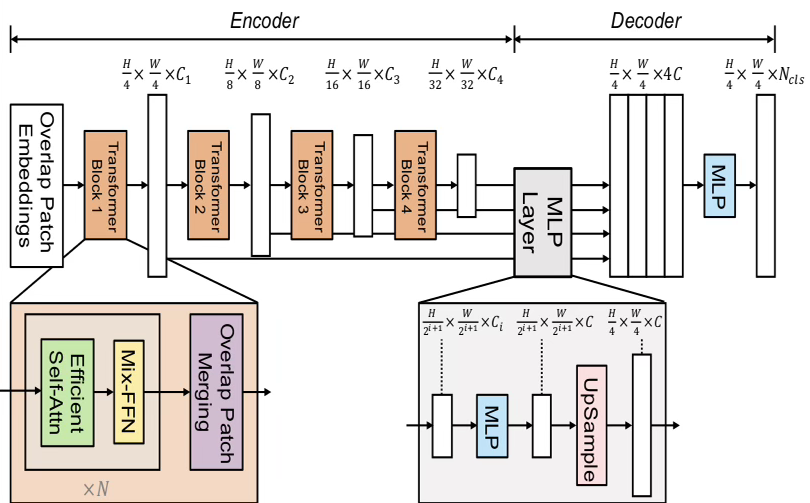
\includegraphics[width=0.78\linewidth]{img/SEGFORMER.png}
    \caption{Архитектура SegFormer}
    \label{fig:segformer}
\end{figure}

\newpage
\section{Сегментатор DeepLabV3+ ResNet101}

\subsection{Архитектура ResNet101}
Энкодер DeepLabV3+ построен на основе сети ResNet-101, глубокой свёрточной сети с остаточными связями (residual connections). Основная идея ResNet - обучение остаточного отображения вместо прямого: если целевое отображение для слоя есть $H(\mathbf{x})$, блок обучает разность $F(\mathbf{x}) = H(\mathbf{x}) - \mathbf{x}$, а выход формируется как $\mathbf{x}_{l+1} = f(\mathbf{x}_l + F(\mathbf{x}_l, \mathcal{W}_l))$, где $f$ - функция активации (ReLU), $\mathcal{W}_l$ - параметры блока. Такая параметризация облегчает обучение очень глубоких сетей и устраняет проблему затухающего градиента.

В ResNet-101 используются \emph{bottleneck}-блоки: остаточная функция $F$ реализована тремя свёртками $1\times 1$, $3\times 3$, $1\times 1$. Обозначив вход блока $\mathbf{x}$, промежуточные выходы после batch normalization и ReLU имеем:
\begin{equation}
\mathbf{z}_1 = \sigma(\mathrm{BN}(W_1 * \mathbf{x})),\quad
\mathbf{z}_2 = \sigma(\mathrm{BN}(W_2 * \mathbf{z}_1)),\quad
F(\mathbf{x}) = W_3 * \mathbf{z}_2,
\end{equation}
где $*$ - свёртка, $\sigma$ - ReLU. Выход блока: $\mathbf{x}_{l+1} = \sigma(\mathbf{x}_l + F(\mathbf{x}_l))$ при совпадении размерностей; при смене разрешения или числа каналов вход проецируется свёрткой $1\times 1$ со stride: $\mathbf{x}_{l+1} = \sigma(\mathrm{Proj}(\mathbf{x}_l) + F(\mathbf{x}_l))$.

Сеть ResNet-101 состоит из начального слоя (свёртка $7\times 7$, max pooling) и трех стадий (conv2\_x  - conv5\_x) с числом блоков 3, 4, 23 соответственно. На первой подстадии каждой стадии пространственное разрешение при необходимости уменьшается в 2 раза (в первой свёртке $3\times 3$ или в проекции), число каналов увеличивается (64, 128, 256, 512). В DeepLabV3+ последние блоки (например, в conv4\_x и conv5\_x) могут использовать атрозные свертки для сохранения плотности карт признаков.

\subsection{Архитектура DeepLabV3+ ResNet101}
Модель DeepLabV3+ с энкодером ResNet-101 объединяет энкодер с модулем ASPP (Atrous Spatial Pyramid Pooling) и декодер для восстановления границ объектов. Главное отличие от обычной свёрточной сети - использование атрозных (разрежённых) свёрток, позволяющих управлять разрешением карт признаков без потери охвата по полю обзора.

Для одномерного сигнала $x[i]$ атрозная свёртка с фильтром $\omega[k]$ длины $K$ и скоростью расширения (dilation rate) $r$ определяется как
\begin{equation}
y[i] = \sum_{k=1}^{K} x[i + r \cdot k] \cdot \omega[k].
\end{equation}
При $r=1$ получается обычная свёртка; при $r>1$ выборка входного сигнала разрежается, что эквивалентно увеличению эффективного поля обзора без роста числа параметров. Для двумерных карт признаков формула обобщается покомпонентно по пространственным индексам. В ResNet-101 при использовании в качестве энкодера DeepLabV3+ атрозные свёртки применяются в последних остаточных блоках для извлечения признаков с заданным output stride (например, 16 или 8).

Модуль ASPP захватывает контекст на нескольких масштабах. Он применяет к выходному тензору backbone несколько параллельных ветвей: свёртку $1\times 1$; три атрозные свёртки $3\times 3$ с разными скоростями расширения $r \in \{6, 12, 18\}$ (при output stride $16$); и ветвь с глобальным усреднением по пространственным координатам (Image-level pooling) для глобального контекста. Выход ASPP - конкатенация результатов всех ветвей, пропущенная через свёртку $1\times 1$ для приведения к 256 каналам:
\begin{equation}
Y_{\mathrm{ASPP}} = \mathrm{Conv}_{1\times 1}\bigl( [f_{1\times 1}(X) \| f_{r=6}(X) \| f_{r=12}(X) \| f_{r=18}(X) \| f_{\mathrm{pool}}(X)] \bigr),
\end{equation}
где $\|$ обозначает конкатенацию по каналам, $f_{\mathrm{pool}}$ - глобальное усреднение с последующей свёрткой $1\times 1$.

В декодере признаки из ASPP сначала апсемплируются билинейной интерполяцией в 4 раза, затем конкатенируются с низкоуровневыми признаками энкодера (например, выход conv2\_x в ResNet-101), предварительно приведёнными к меньшему числу каналов свёрткой $1\times 1$. После конкатенации применяются две свёртки $3\times 3$ с 256 фильтрами для уточнения карт признаков, затем финальный билинейный апсемплинг в 4 раза восстанавливает исходное пространственное разрешение изображения.

В качестве функции потерь используется кросс-энтропия по пикселям:
\begin{equation}
L = -\frac{1}{N} \sum_{i=1}^{N} \sum_{c=1}^{C} y_{i,c} \log \hat{y}_{i,c},
\end{equation}
где $N$ - число пикселей, $C$ - число классов, $y_{i,c}$ - истинная метка (one-hot по классам), $\hat{y}_{i,c}$ - предсказание модели (вероятность класса $c$ в пикселе $i$).

Ниже на рисунке \ref{fig:deeplab} представлена архитектура DeepLabV3+ ResNet101:
\begin{figure}[H]
    \centering
    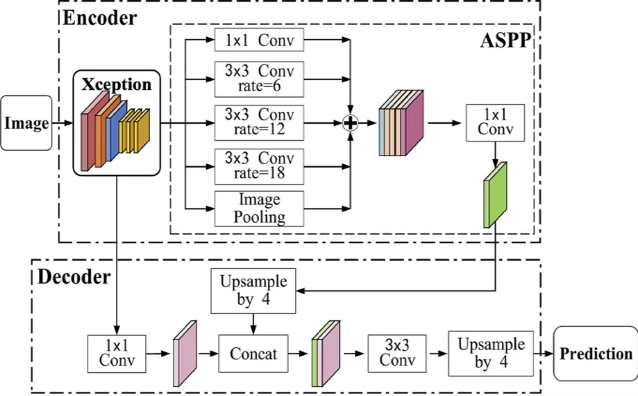
\includegraphics[width=0.78\linewidth]{img/DEEPLAB.png}
    \caption{Архитектура DeepLabV3+}
    \label{fig:deeplab}
\end{figure}

\newpage
\section{Сегментатор YOLO-seg}

Модель YOLO-seg выполняет попиксельную сегментацию: для каждого обнаруженного объекта предсказывается ограничивающий прямоугольник, класс, и пиксельная маска контура. Архитектура совмещает общую часть детектора (backbone, neck, head детекции) с модулем генерации масок по схеме прототипных масок, унаследованной от YOLACT.

Входное изображение проходит через backbone с блоками C3k2 (Cross Stage Partial с ядром 2): разбиение входа на две ветви, одна сохраняется, вторая обрабатывается параллельными свёртками с последующей конкатенацией для эффективного извлечения признаков. Модуль SPPF (Spatial Pyramid Pooling Fast) агрегирует контекст на нескольких масштабах через последовательный max pooling и свёртку. В neck используется блок C2PSA (CSP с Pyramid Squeeze Attention): пространственное внимание с ядрами разного размера и взвешивание каналов. На выходе neck формируется пирамида признаков для head-ов детекции и сегментации.

Детекция выполняется в безякорном формате: для каждой ячейки/позиции предсказываются смещения центра объекта $(t_x, t_y)$, размеры $(t_w, t_h)$, оценка объектности и распределение по классам. После декодирования координат и пороговой фильтрации получают множество детекций $\mathcal{D} = \{(b_i, c_i, s_i)\}$, где $b_i$ - бокс, $c_i$ - класс, $s_i$ - уверенность.

Сегментация добавляет к каждой детекции маску. Модель выдаёт два типа выходов:
\begin{itemize}
    \item \textbf{Прототипные маски} $\mathbf{P}$: тензор размерности $n_m \times H_p \times W_p$ ($n_m = 32$ в стандартной конфигурации), получаемый отдельной свёрточной ветвью (ProtoNet) от карт признаков neck. Каждый канал $P_k(h,w)$ интерпретируется как базисная пространственная карта.
    \item \textbf{Коэффициенты масок}: для каждой детекции $i$ head предсказывает вектор $\mathbf{a}_i = (a_{i1}, \ldots, a_{i,n_m})^\top \in \mathbb{R}^{n_m}$ (дополнительные каналы в выходе head детекции).
\end{itemize}

Итоговая маска для детекции $i$ формируется как линейная комбинация прототипов с последующей поэлементной сигмоидой:
\begin{equation}
\tilde{M}_i(h,w) = \sigma\biggl( \sum_{k=1}^{n_m} a_{ik} \cdot P_k(h,w) \biggr),
\quad \sigma(z) = \frac{1}{1 + e^{-z}},
\end{equation}
где $(h,w)$ - координаты в сетке прототипов размера $H_p \times W_p$. В матричной форме: пусть $\mathbf{P} \in \mathbb{R}^{n_m \times (H_p W_p)}$ - прототипы, развёрнутые по пространственным индексам; тогда вектор логитов маски для детекции $i$ есть $\mathbf{a}_i^\top \mathbf{P}$, после $\sigma$ и обратного преобразования в форму $H_p \times W_p$ получают $\tilde{M}_i$. Далее маску обрезают по ограничивающему прямоугольнику детекции $b_i$, при необходимости бинаризуют по порогу (например, $0.5$) и масштабируют до размера кадра или бокса для получения финальной пиксельной маски $M_i$.

На выходе сегментатора для каждого объекта имеем тройку $(b_i, c_i, M_i)$: бокс, класс и маска контура. Обучение сегментации ведётся совместно с детекцией; в функцию потерь входят слагаемые для боксов, классификации и для масок (например, бинарная кросс-энтропия или dice между предсказанной и целевой маской в области объекта).

Ниже на рисунке \ref{fig:yoloseg} представлена архитектура YOLO-seg:
\begin{figure}[H]
    \centering
    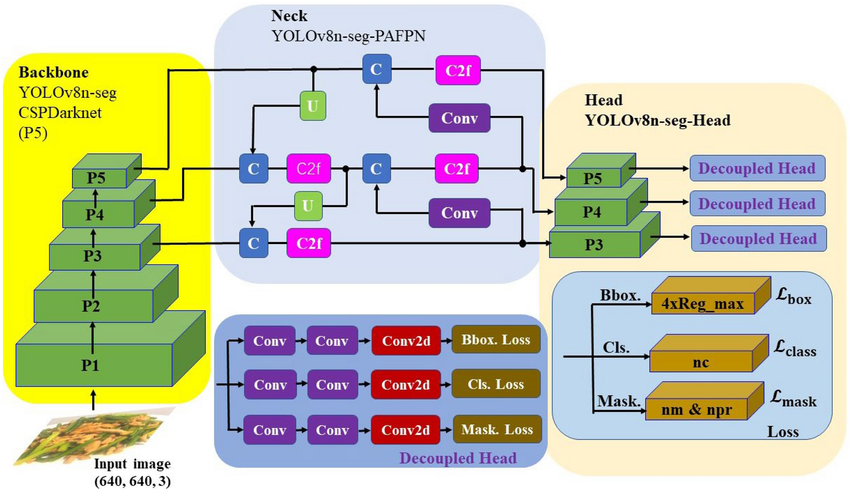
\includegraphics[width=0.78\linewidth]{img/YOLO.png}
    \caption{Архитектура YOLO-seg на примере YOLOv8n-seg}
    \label{fig:yoloseg}
\end{figure}

\newpage
\section{Подготовка датасета}

В качестве выборки для обучения выбран открытый датасет RailSem19: семантическая сегментация сцен железнодорожной инфраструктуры. Датасет содержит 8500 изображений с пиксельной разметкой. В состав входят: сами изображения; разметка в формате JSON; маски в формате \textbf{uint8}; конфигурационный JSON с объявлением классов.

Маска семантической сегментации хранится как одноканальное изображение, в котором каждому пикселю соответствует один байт (тип \texttt{uint8}) - индекс класса. Значение пикселя $p(h,w) \in \{0, 1, \ldots, N_{\mathrm{cls}}-1\}$ указывает принадлежность пикселя $(h,w)$ одному из $N_{\mathrm{cls}}$ классов; при $N_{\mathrm{cls}} \leq 256$ одного байта достаточно. Такой формат компактен по памяти (один байт на пиксель вместо трёх каналов в RGB-маске), удобен для многоклассовой сегментации и напрямую подходит для обучения моделей типа SegFormer или DeepLabV3+: функция потерь (кросс-энтропия) ожидает на входах целочисленные метки классов по пикселям. В RailSem19 маски в uint8 позволяют однозначно задать семантическую разметку для всех 19 классов.

В датасете используется 19 классов, объединённых в три группы: рельсы (5 классов), городская среда (11 классов), транспорт (4 класса). Конфигурационный JSON задаёт соответствие между индексами и именами классов и используется при загрузке разметки и при конвертации в другие форматы.

Обучение модели YOLO-seg на таких данных в исходном виде невозможно из-за различия форматов. Каждый объект задаётся отдельно, разметка хранится в текстовых файлах (один \texttt{.txt} на изображение), в каждой строке - один объект в виде
\begin{center}
\texttt{<класс> <x\_1> <y\_1> <x\_2> <y\_2> \ldots <x\_n> <y\_n>},
\end{center}
где координаты $(x_i, y_i)$ - вершины полигона контура объекта в нормализованных координатах (относительно ширины и высоты изображения, значения в $[0, 1]$). Минимум три точки на объект; число вершин у разных объектов может отличаться. Таким образом, YOLO-seg ожидает не пиксельную карту классов (uint8 маску), а список полигонов по объектам. При обучении контур каждого объекта по этим вершинам растеризуется в бинарную маску в области ограничивающего прямоугольника; по этой маске считается слагаемое потерь для масок (например, бинарная кросс-энтропия или dice). Итоговая маска на инференсе строится из прототипов и коэффициентов; формат разметки при обучении - именно полигоны, чтобы компактно хранить контуры и однозначно сопоставлять каждую маску конкретному объекту (детекции).

Для приведения датасета RailSem19 к формату, пригодному для обучения YOLO-seg, используется репозиторий JSON2YOLO от Ultralytics. Он автоматически преобразует исходные аннотации (JSON и маски) в структуру каталогов с подпапками \texttt{images/} и \texttt{labels/}: для каждого изображения создаётся текстовый файл с тем же именем, в котором для каждого объекта указаны индекс класса и нормализованные координаты вершин полигона в одну строку. Дополнительно задаётся YAML-конфигурация датасета с путями к \texttt{train/} и \texttt{val/} и словарём имён классов. После конвертации датасет можно использовать для обучения YOLO-seg и оценки качества сегментации в формате попиксельной сегментации.

Ниже представлен пример кода конвертации датасета на основе JSON, в формат обучения YOLO:

За основу берется метод convert\_coco из библиотеки ultralytics.

\begin{lstlisting}
    from ultralytics.data.converter import convert_coco

    convert_coco(
    labels_dir='PATH/to/annotations/',  
    use_segments=True                   
    )
\end{lstlisting}

\newpage
\section{Стандартное обучение сегментаторов}
Под стандартным обучением в работе, понимается стандартное деление датасета на обучающую, валидационную и тестовую части выборки. В последствие для выборанной модели сегментатора, будет использватся кросс-валидация с методом leave one  out. 

Подбор гиперпараметров средствами Optune - долгая и тяжеловесная задача для видеопамяти. Было принято решение использовать более легкий метод подбора гиперпараметров методом tune, который предоставляет ultralytics для моделей YOLO-seg.

\subsection{Генетический алгоритм tune}
Метод tune от ultralytics представляет собой эволюционный алгоритм, направленный на максимизацию метрик качества модели $mAP$, $accuracy$ и других метрик в зависимости от модели. 
В основе процесса лежит использование библиотеки Ray Tune, для перебора пространства гиперпараметров. 

Формально настройка гиперпараметров - задача оптимизации:

$$
    \theta^* = \arg \max_{\theta \in \Theta} F(M(\theta), D_{val}),
$$

где $\theta$ - вектор гиперпараметров, $\Theta$ - пространство поиска (диапазон допустимых значений для гиперпараметров), 
$M(\theta)$ - модель сегментатора обучающаяся на векторе $\theta$, $D_val$ - валидационный набор данных, $F$ - целевая функция (основная метрика максимизации),
$\theta^*$ - оптимальный набор гиперпараметров.

Во время каждой эволюции (trial), внутри настройки модель оптимизирует веса $\omega$ через функцию потерь $ \mathcal{L}$

Модель YOLO, имеет единый прогон по нейросети которая: выделяет, классифцирует, заносит в рамки сегмент, и выглядит как сумма всех функций потерь:
$$
     \mathcal{L}_{total} = \lambda_1  \mathcal{L}_{seg} + \lambda_2  \mathcal{L}_{cls} + \lambda_3  \mathcal{L}_{box}
$$

где коэффициенты $\lambda_i$ - так же могут настраиватся.

Чтобы алгоритм выявлял лучшее решение, задается взвешанная сумма метрик, которая является скалярным произведением вектора 
результатов на результаты весов:

$$
    F(h) = \sum_{i=1}^{n} w_i \cdot m_i
$$

В YOLO-seg, фитнес функция задается как $F = 0.1 \cdot mAP@50 + 0.9 \cdot mAP@50 - 95$.

Инициализация происходит следующим образом:

$N$ - набор гиперпараметров, на каждой итерации алгоритм выбирает $k$ - лучших родителей у котолрых значение $F(h) = argmax F(h)$, 
остальные особи отбрасываются.

Новое поколение создается оператором мутации путем добавления случайного шума к параметрам лучших родителей:

$$
    \forall h_j : h_{j}^{new} = h_{j}^{parent} \cdot M
$$

$M$ - множетель мутации определяется через распределение: 
$$
    M = clip(1 +  \mathcal{N}(0, \sigma^2), min, max),
$$
где $\sigma$ - коэффициент интенсивности мутации с затуханием, $clip$ - функция ограничения чтобы параметр не вышел за границы (например что бы псевдо-вероятность не привышала 1).

Кроссовер как скрещивание двух родителей выгледит как линейная комбинация двух родителей $P_1$, $P_2$: 
$$
    h^{child} = \alpha P_1 + (1-\alpha)P_2
$$
При этом, $\alpha$ случайное число. В итоге ребенок наследует каждый ген (параметр) от одного из родителей с вероятности $\frac{1}{2}$.

Итерации при этом являются цепью Маркова, где следующее состояние популяции $H_{t+1}$ зависит от текущего $H_t$

Вычисляется $F(h_i) \forall i \in {1,\dots, N}$, далее идет сортировка такая что $F(h_1) \geq F(h_2) \geq \dots \geq F(h_N)$,
тогда следующий $h_{i}^{t+1} = Mutate(Select(H_t))$. Останова происходит либо вручную пока $t = T$, либо по заданной точности $\varepsilon$.

Для реализации подбора гиперпараметров, необходимо воспользоватся библиотекой ultralytics:

\begin{lstlisting}
    from ultralytics import YOLO

    model = YOLO("yolo11s-seg.pt")
    
    results = model.tune(
        data="PATH",        
        epochs=30,        
        iterations=100,     
        optimizer="AdamW",    # OPTIMIZER
        plots=False,   
        save=False,    
        val=True      
    )
\end{lstlisting}

\subsection{Результаты подбора гиперпараметров}
По результатам подбора, использовалось 30 эпох на 20 поколений, что заняло 35 часов. На рисунке \ref{fig:hyper}, представлены диаграммы рассеивания гиперпараметров.
Черный крестик, обозначает лучший гиперпараметр из всех использванных.  

\begin{figure}[H]
    \centering
    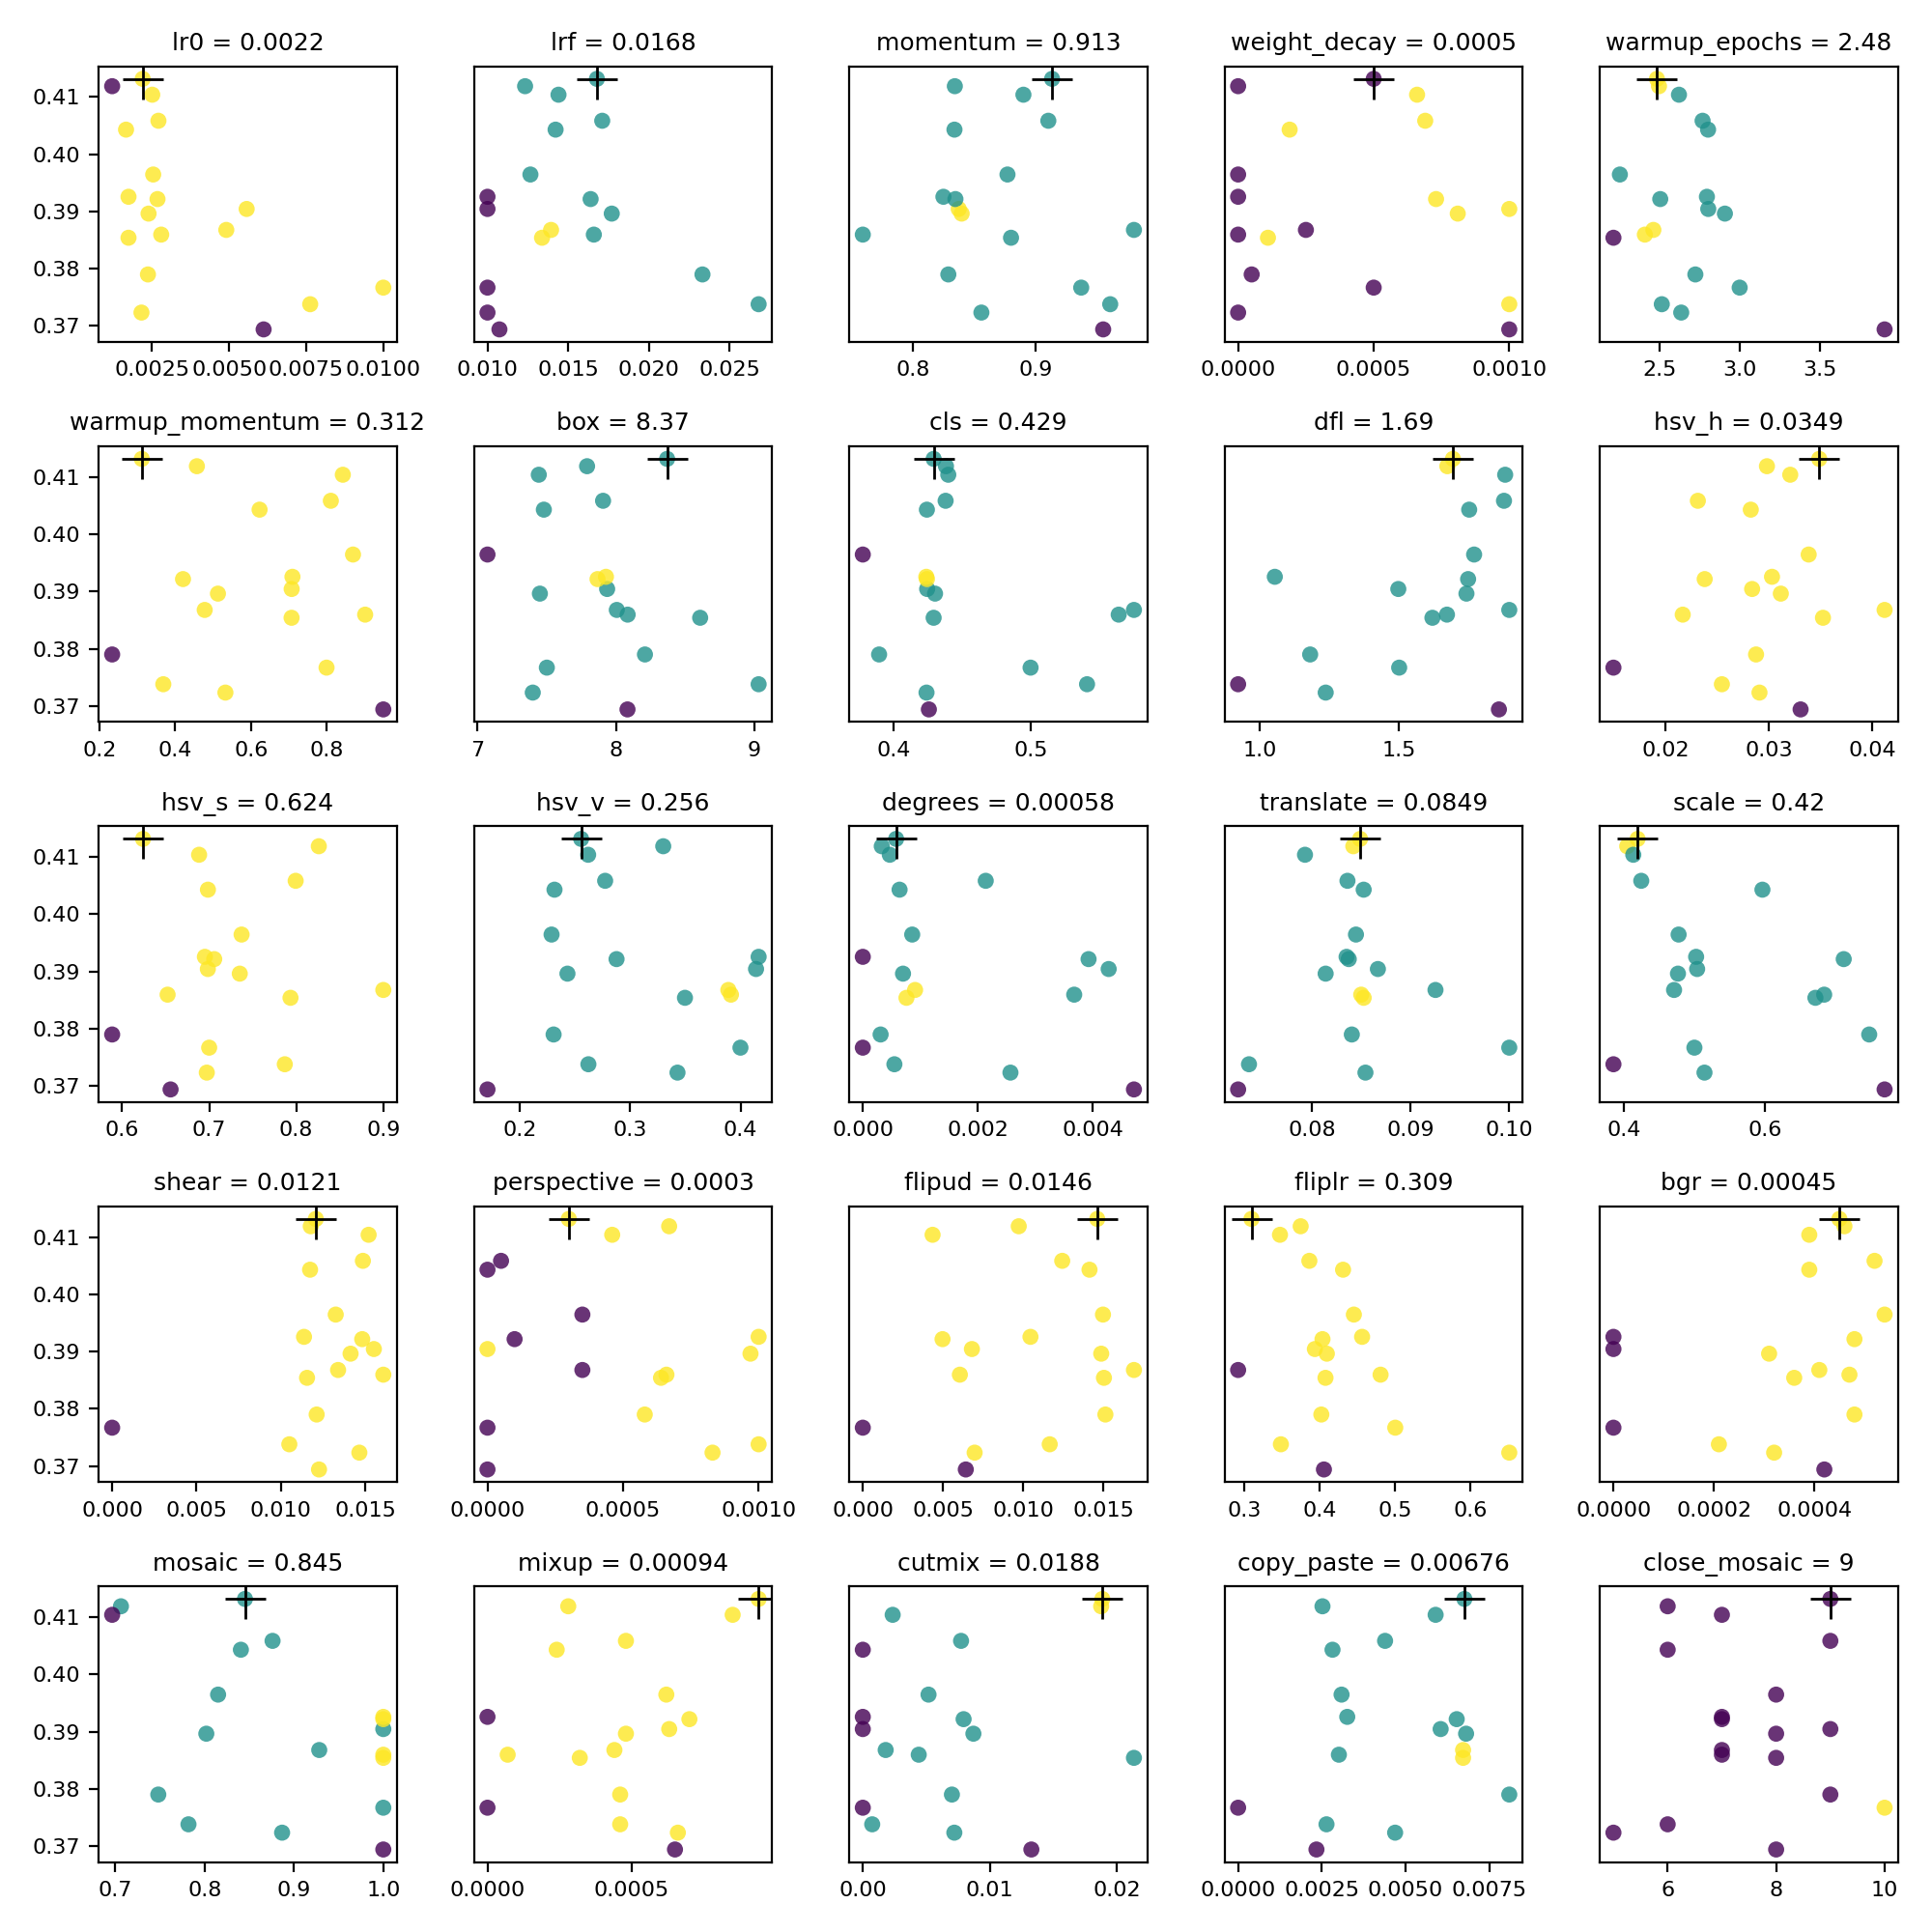
\includegraphics[width=0.68\linewidth]{img/TUNE.png}
    \caption{Результаты подбора гиперпараметров}
    \label{fig:hyper}
\end{figure}

Ниже в таблице \ref{tab:hyper1} представлены полученные гиперпараметры для обучения

\begin{table}[H]
\centering
\caption{Таблица 1. Полученные гиперпараметры (часть 1)}
\label{tab:hyper1}
\resizebox{\textwidth}{!}{%
\scriptsize
\begin{tabular}{|r|r|r|r|r|r|r|r|r|r|r|r|r|r|r}
\hline
№ & fit & lr0 & lrf & mom & wd & warmEp & warmMom & box & cls & dfl & hsv\_h & hsv\_s & hsv\_v & deg \\
\hline
1 & 0.377 & 0.010 & 0.010 & 0.937 & 0.0005 & 3.0 & 0.80 & 7.50 & 0.50 & 1.50 & 0.015 & 0.70 & 0.40 & 0.0 \\
2 & 0.390 & 0.0056 & 0.010 & 0.837 & 0.001 & 2.80 & 0.71 & 7.94 & 0.42 & 1.50 & 0.028 & 0.70 & 0.41 & 0.004 \\
3 & 0.393 & 0.0017 & 0.010 & 0.825 & 0.0 & 2.79 & 0.71 & 7.93 & 0.42 & 1.05 & 0.030 & 0.70 & 0.42 & 0.0 \\
4 & 0.404 & 0.0017 & 0.014 & 0.834 & 0.0002 & 2.80 & 0.62 & 7.48 & 0.42 & 1.75 & 0.028 & 0.70 & 0.23 & 0.001 \\
5 & 0.412 & 0.0012 & 0.012 & 0.834 & 0.0 & 2.49 & 0.46 & 7.79 & 0.44 & 1.67 & 0.030 & 0.83 & 0.33 & 0.0003 \\
6 & 0.372 & 0.0022 & 0.010 & 0.856 & 0.0 & 2.63 & 0.53 & 7.40 & 0.42 & 1.24 & 0.029 & 0.70 & 0.34 & 0.003 \\
7 & 0.392 & 0.0027 & 0.016 & 0.834 & 0.0007 & 2.50 & 0.42 & 7.87 & 0.42 & 1.75 & 0.024 & 0.71 & 0.29 & 0.004 \\
\textcolor{red}{8} & \textcolor{red}{0.413} & \textcolor{red}{0.0022} & \textcolor{red}{0.017} & \textcolor{red}{0.913} & \textcolor{red}{0.0005} & \textcolor{red}{2.48} & \textcolor{red}{0.31} & \textcolor{red}{8.37} & \textcolor{red}{0.43} & \textcolor{red}{1.69} & \textcolor{red}{0.035} & \textcolor{red}{0.62} & \textcolor{red}{0.26} & \textcolor{red}{0.001} \\
9 & 0.406 & 0.0027 & 0.017 & 0.910 & 0.0007 & 2.77 & 0.81 & 7.91 & 0.44 & 1.88 & 0.023 & 0.80 & 0.28 & 0.002 \\
10 & 0.374 & 0.0076 & 0.027 & 0.961 & 0.001 & 2.51 & 0.37 & 9.03 & 0.54 & 0.92 & 0.025 & 0.79 & 0.26 & 0.001 \\
11 & 0.387 & 0.0049 & 0.014 & 0.98 & 0.0003 & 2.46 & 0.48 & 8.01 & 0.58 & 1.90 & 0.041 & 0.90 & 0.39 & 0.001 \\
12 & 0.390 & 0.0024 & 0.018 & 0.840 & 0.0008 & 2.91 & 0.51 & 7.45 & 0.43 & 1.74 & 0.031 & 0.74 & 0.24 & 0.001 \\
13 & 0.386 & 0.0028 & 0.017 & 0.759 & 0.0 & 2.41 & 0.90 & 8.08 & 0.56 & 1.67 & 0.022 & 0.65 & 0.39 & 0.004 \\
14 & 0.379 & 0.0024 & 0.023 & 0.829 & 0.0001 & 2.72 & 0.23 & 8.21 & 0.39 & 1.18 & 0.029 & 0.59 & 0.23 & 0.0003 \\
15 & 0.369 & 0.0061 & 0.011 & 0.955 & 0.001 & 3.91 & 0.95 & 8.08 & 0.43 & 1.86 & 0.033 & 0.66 & 0.17 & 0.005 \\
16 & 0.410 & 0.0025 & 0.014 & 0.890 & 0.0007 & 2.62 & 0.84 & 7.44 & 0.44 & 1.88 & 0.032 & 0.69 & 0.26 & 0.0005 \\
17 & 0.0 & 0.0021 & 0.012 & 0.925 & 0.0 & 2.56 & 0.41 & 4.72 & 0.44 & 2.39 & 0.034 & 0.80 & 0.22 & 0.0003 \\
18 & 0.396 & 0.0025 & 0.013 & 0.877 & 0.0 & 2.25 & 0.87 & 7.07 & 0.38 & 1.77 & 0.034 & 0.74 & 0.23 & 0.001 \\
19 & 0.385 & 0.0017 & 0.013 & 0.880 & 0.0001 & 2.21 & 0.71 & 8.61 & 0.43 & 1.62 & 0.035 & 0.79 & 0.35 & 0.001 \\
20 & 0.0 & 0.0017 & 0.014 & 0.851 & 0.0001 & 2.96 & 0.89 & 7.09 & 0.45 & 2.06 & 0.033 & 0.64 & 0.32 & 0.002 \\
\hline
\end{tabular}%
}
\end{table}

\begin{table}[H]
\centering
\label{tab:hyper2}
\resizebox{\textwidth}{!}{%
\scriptsize
\begin{tabular}{r|r|r|r|r|r|r|r|r|r|r|r|r|}
\hline
№ & transl & scale & shear & persp & flipud & fliplr & bgr & mosaic & mixup & cutmix & copy\_p & close \\
\hline
1 & 0.10 & 0.50 & 0.0 & 0.0 & 0.0 & 0.50 & 0.0 & 1.0 & 0.0 & 0.0 & 0.0 & 10 \\
2 & 0.087 & 0.50 & 0.016 & 0.0 & 0.007 & 0.39 & 0.0 & 1.0 & 0.0006 & 0.0 & 0.006 & 9 \\
3 & 0.084 & 0.50 & 0.011 & 0.001 & 0.010 & 0.46 & 0.0 & 1.0 & 0.0 & 0.0 & 0.003 & 7 \\
4 & 0.085 & 0.60 & 0.012 & 0.0 & 0.014 & 0.43 & 0.0004 & 0.84 & 0.0002 & 0.0 & 0.003 & 6 \\
5 & 0.084 & 0.41 & 0.012 & 0.001 & 0.010 & 0.37 & 0.0005 & 0.71 & 0.0003 & 0.019 & 0.003 & 6 \\
6 & 0.085 & 0.51 & 0.015 & 0.001 & 0.007 & 0.65 & 0.0003 & 0.89 & 0.0007 & 0.007 & 0.005 & 5 \\
7 & 0.084 & 0.71 & 0.015 & 0.0001 & 0.005 & 0.40 & 0.0005 & 1.0 & 0.0007 & 0.008 & 0.007 & 7 \\
\textcolor{red}{8} & \textcolor{red}{0.085} & \textcolor{red}{0.42} & \textcolor{red}{0.012} & \textcolor{red}{0.0003} & \textcolor{red}{0.015} & \textcolor{red}{0.31} & \textcolor{red}{0.0005} & \textcolor{red}{0.85} & \textcolor{red}{0.0009} & \textcolor{red}{0.019} & \textcolor{red}{0.007} & \textcolor{red}{9} \\
9 & 0.084 & 0.42 & 0.015 & 0.0001 & 0.012 & 0.39 & 0.0005 & 0.88 & 0.0005 & 0.008 & 0.004 & 9 \\
10 & 0.074 & 0.39 & 0.011 & 0.001 & 0.012 & 0.35 & 0.0002 & 0.78 & 0.0005 & 0.001 & 0.003 & 6 \\
11 & 0.093 & 0.47 & 0.013 & 0.0004 & 0.017 & 0.29 & 0.0004 & 0.93 & 0.0004 & 0.002 & 0.007 & 7 \\
12 & 0.081 & 0.48 & 0.014 & 0.001 & 0.015 & 0.41 & 0.0003 & 0.80 & 0.0005 & 0.009 & 0.007 & 8 \\
13 & 0.085 & 0.68 & 0.016 & 0.001 & 0.006 & 0.48 & 0.0005 & 1.0 & 0.0001 & 0.004 & 0.003 & 7 \\
14 & 0.084 & 0.75 & 0.012 & 0.001 & 0.015 & 0.40 & 0.0005 & 0.75 & 0.0005 & 0.007 & 0.008 & 9 \\
15 & 0.073 & 0.77 & 0.012 & 0.0 & 0.006 & 0.41 & 0.0004 & 1.0 & 0.0007 & 0.013 & 0.002 & 8 \\
16 & 0.079 & 0.41 & 0.015 & 0.0005 & 0.004 & 0.35 & 0.0004 & 0.70 & 0.0009 & 0.002 & 0.006 & 7 \\
17 & 0.090 & 0.45 & 0.012 & 0.001 & 0.010 & 0.36 & 0.0004 & 0.50 & 0.0008 & 0.010 & 0.007 & 6 \\
18 & 0.084 & 0.48 & 0.013 & 0.0004 & 0.015 & 0.45 & 0.0005 & 0.82 & 0.0006 & 0.005 & 0.003 & 8 \\
19 & 0.085 & 0.67 & 0.012 & 0.001 & 0.015 & 0.41 & 0.0004 & 1.0 & 0.0003 & 0.021 & 0.007 & 8 \\
20 & 0.086 & 0.61 & 0.018 & 0.0 & 0.004 & 0.43 & 0.0007 & 0.66 & 0.0003 & 0.013 & 0.006 & 8 \\
\hline
\end{tabular}%
}
\end{table}

\noindent Обозначения: fit - fitness; lr0, lrf - параметры learning rate; mom - momentum; wd - weight decay; warmEp, warmMom - warmup; box, cls, dfl - веса потерь; hsv\_h/s/v - аугментация HSV; deg - degrees; transl - translate; persp - perspective; copy\_p - copy\_paste; close - close\_mosaic.

Окончательные результаты гиперпараметров представлены в таблице \ref{tab:finalHyper}:

\begin{table}[H]
\centering
\caption{Лучший результат из подбора гиперпараметров}
\label{tab:finalHyper}
\footnotesize
\begin{tabular}{|ll|ll|ll|}
\hline
Параметр & Значение & Параметр & Значение & Параметр & Значение \\
\hline
lr0 & 0.0022 & lrf & 0.01678 & momentum & 0.91324 \\
weight\_decay & 0.0005 & warmup\_epochs & 2.48151 & warmup\_momentum & 0.31178 \\
box & 8.369 & cls & 0.42917 & dfl & 1.69298 \\
hsv\_h & 0.03487 & hsv\_s & 0.62407 & hsv\_v & 0.25582 \\
degrees & 0.00058 & translate & 0.0849 & scale & 0.41977 \\
shear & 0.01207 & perspective & 0.0003 & flipud & 0.01461 \\
fliplr & 0.30946 & bgr & 0.00045 & mosaic & 0.8451 \\
mixup & 0.00094 & cutmix & 0.01884 & copy\_paste & 0.00676 \\
close\_mosaic & 9 & & & & \\
\hline
\end{tabular}
\end{table}

\subsection{Выбор метода оптимизации}
Подбор гиперпараметров, касаются архитектуры моделей ultralytics, эти параметры будут использвованы для обучения и выбора модели между версиями и конфигурациями YOLO-seg:
\begin{itemize}
    \item YOLOv8n-seg;
    \item YOLOv8s-seg;
    \item YOLOv11s-seg;
    \item YOLO26s-seg.
\end{itemize}

Модель YOLOv8n-seg, является самой легковесной моделью, которая ориентирована на мобильные устройства. 
YOLOv8s-seg, тяжелее относительно YOLOv8n-seg, но она так же ориентирована на мобильные устройства с более мощным аппаратным обеспечением.
Модель YOLOv11s-seg, является более продвинутой моделью относительно YOLOv8s-seg, использующая более мощный и оптимизированный энкодер.
YOLO26s-seg, современная модель, вышедшая в 2026 году, однако из источников, сообщается о том, что модель не ориентирована на специфические датасеты, и более
ориентирована на датасет типа COCO, которую используют ultralytics, для оценки точности модели.

Для реализации обучения, изначально к гиперпараметрам, необходимо подобрать метод оптимизации минимизации функции потерь, так как этот метод будет использоваться для обучения всех моделей.

\subsection{Эволюционный алгоритм CMA-ES}
В расматриваемых вариантах для минимизации из генетических алгоритмов, был выбран алгоритм CMA-ES. 

CMA-ES (Covarianc Matrix Adaptation - Evolution Strategy) - это итеративный стахостический алгоритм оптимизации второго порядка, для поиска минимума в сложных пространствах.

Входными данными алгоритма являются:
\begin{itemize}
    \item Целевая функция которую необходимо минимизировать - это функция потерь;
    \item Начальная точка: $m \in \mathbb{R}^n$ - центр распределения (начальное приблежение);
    \item Начальный шаг: $\sigma \in \mathbb{R}_+$ - размер области поиска;
    \item Размер популяции: $\lambda$ - количество точек генерируемых в каждой итерации;
\end{itemize}

Основной цикл, состоит из пяти частей - в начале генерируется $\lambda$ векторов из многомерного нормального распределения $x_k \sim \mathcal{N}(0,C)$, где $C$ - ковариационная матрица.

Далее вычисляются значения целевой функции $f(x_k)$, для всех точек. Точки сортируются по значению, и отбираются $\mu \approx \frac{\lambda}{2}$ лучших кандидатов.

После вычисляется среднее значение $m$, как взвешенная сумма лучших точек, что позволяет смещать центр поиска в окрестности минимума.

Если последовательные шаги среднего значения сонаправлены, то $\sigma$ увеличивается и алгоритм ускоряется, если шаги \guillemetleft гасят\guillemetright друг друга, 
то $\sigma$ уменьшается, что означает, что алгоритм сходится.

Матрица $C$, обнавляется так, что бы увеличить вероятность генерации точек в направлениях где ранее было достигнуто лучшее значение. 
Таким образом пространство поиска диформируется в вытянутый эллипсоид, оси которого соответствуют собственным векторам $C$. Процесс является аппроксимацией обратной матрицы Гесса.

На выходе, алгоритм возвращает вектор $x_k$, который является точкой минимума функции потерь, а матрица $C$ описывает локальную структуру функции.

На рисунке \ref{fig:CMA}, изображена блок-схема алгоритма:

\begin{figure}[H]
    \centering 
    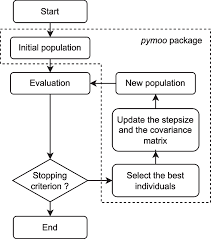
\includegraphics[width=0.48\linewidth]{img/CMA_ES.png}
    \caption{Блок-схема CMA-ES}
    \label{fig:CMA}
\end{figure}

Сложность алгоритма состовляет по памяти $O(n^2)$, где $n$ - количество параметров. 

Модель YOLOv8n-seg, хоть и является самой маленькой моделью, но имеет 3.4 милионов параметров. Что означает, 
что при классической реализации алгоритма CMA-ES, в VRAM, придется хранить $\approx 3400000^2 \approx 11560000000000$ параметров.
В теории, данный алгоритм при инициализации популяции, должен быть прерван на стадии инициализации. 
На практике можно применить оптимизированный алгоритм CMA-ES, из библиотеки torch - eye.

Для начала нужно сформировать вектор из параметров модели YOLOv8s-seg:

\begin{lstlisting}
    import torch
    import numpy as np
    from ultralytics import YOLO

    model = YOLO("yolov8n-seg.pt")
    
    trainable_params = [p for p in model.model.parameters() if p.requires_grad]
    N = sum(p.numel() for p in trainable_params)

    try:
        m = torch.cat([p.view(-1) for p in trainable_params]).detach().numpy()
        C = np.eye(N, dtype=np.float32)
    except MemmoryError:
        print("Ooops! Out of Memmory")    
\end{lstlisting}

Результатом вывода оказалось строка: \guillemetleft Ooops! Out of Memmory\guillemetright, 
что подверждает, что памяти не хватит под модели обучения. 

Для реализации минимизации функции потерь на практике используются методы градиентного спуска: стахостический градиентный спуск либо адаптивная оценка моментов с разделенным распадом весов (AdamW).

\subsection{SGD}
Метод SGD - стахостический градиентный спуск, основан на обнавлении весов по направлению антиградиента:

$$
    \theta_{t+1} = \theta_t - \eta \cdot \nabla f(\theta_t)
$$

При этом в YOLO используется добавление инерции, для ускарения спуска (этот метод является инерционным). При этом алгоритм становится таким:

\begin{itemize}
    \item $v_{t+1} = \mu v_t + \nabla f(\theta_t)$
    \item $\theta_{t+1} = \theta_t - \eta v_{t+1}$
\end{itemize}

Где $\mu$ - коэффициент инерции, $\eta$ - скорость обучения (learning rate в ultralytics).

\subsection{AdamW}

Данный метод, вычисляет индивидуальный шаг обучения для каждого параметра, используя оценки первого и второго момента градиента.

Алгоритм выглядит следующим образом:
\begin{itemize}
    \item Обнавление моментов: \begin{enumerate} 
        \item $m_t = \beta_1 m_{t-1} + (1 - \beta_1) \nabla f(\theta_t)$ - среднее значение градиента
        \item $v_t = \beta_2 v_{t-1} + (1 - \beta_2)(\nabla f(\theta_t))^2$ - дисперсия
    \end{enumerate}
    \item Корректировка смещения: $\hat{m}_t = \frac{m_t}{1 - \beta_1^t}$ и $\hat{v}_t = \frac{v_t}{1 - \beta_2^t}$
    \item Обнавление весов: $\theta_{t+1} = \theta_t - \eta \cdot \frac{\hat{m}_t}{\sqrt{\hat{v}_t} + \epsilon}$
\end{itemize}

Теоретически, метод AdamW является более точным, чем SGD, хотя и более ресурсоемкий.

Принято решение использовать метод AdamW, для обеспечения более точной минимизации функции потерь.

\newpage
\section{Обучение сегментаторов}
Для реализации обучения сегментаторов, используется библиотека ultralytics, 
для этого используется метод train() из библиотеки, которая принимает на вход полученные 
гиперпараметры из главы 8.2.

Для начала нужно импортировать необходимые библиотеки, и объявить константы для разбиения датасета на
данные для обучения, валидации и тестирования.

\begin{lstlisting}
    import os
    import random
    import yaml
    from pathlib import Path
    from ultralytics import YOLO, settings
    
    os.environ["TORCH_FORCE_WEIGHTS_ONLY_LOAD"] = "0"
    
    _SCRIPT_DIR = Path(__file__).resolve().parent
    DIR_YOLO_DATASET = _SCRIPT_DIR / "yolo_dataset"
    DATA_YAML = DIR_YOLO_DATASET / "data.yaml"
    YOLO_DATA_PATH = DIR_YOLO_DATASET
    IMG_SRC = None
    LBL_SRC = None
    
    TRAIN_SIZE = 7000
    VAL_SIZE = 1000
    TEST_SIZE = 500
\end{lstlisting}

После чего необходимо создать словарь для объявления классов и их индексов:

\begin{lstlisting}
    CLASS_NAMES = {
        0: "road", 1: "sidewalk", 2: "construction", 3: "tram-track", 4: "fence",
        5: "pole", 6: "traffic-light", 7: "traffic-sign", 8: "vegetation", 9: "terrain",
        10: "sky", 11: "human", 12: "rail-track", 13: "car", 14: "truck",
        15: "trackbed", 16: "on-rails", 17: "rail-raised", 18: "rail-embedded",
    }
\end{lstlisting}

Далее реализуется метод для разбиения датасета на данные для обучения, валидации и тестирования:
\begin{lstlisting}
    def _resolve_data_paths():
    global IMG_SRC, LBL_SRC
    if IMG_SRC is not None and LBL_SRC is not None:
        return
    exts = (".jpg", ".jpeg", ".png", ".bmp")
    if DATA_YAML.exists():
        with open(DATA_YAML, encoding="utf-8") as f:
            cfg = yaml.safe_load(f)
        base = Path(cfg.get("path", "."))
        if not base.is_absolute():
            base = (DATA_YAML.parent / base).resolve()
        train_rel = cfg.get("train", "images/rs19_val")
        img_dir = base / train_rel
        lbl_dir = base / "labels" / Path(train_rel).name
        if img_dir.is_dir() and lbl_dir.is_dir():
            n = [f.stem for f in lbl_dir.glob("*.txt") if any((img_dir / f"{f.stem}{e}").exists() for e in exts)]
            if n:
                IMG_SRC = img_dir
                LBL_SRC = lbl_dir
                return
    for part in ("rs19_val", "train"):
        img_dir = DIR_YOLO_DATASET / "images" / part
        lbl_dir = DIR_YOLO_DATASET / "labels" / part
        if img_dir.is_dir() and lbl_dir.is_dir():
            n = [f.stem for f in lbl_dir.glob("*.txt") if any((img_dir / f"{f.stem}{e}").exists() for e in exts)]
            if n:
                IMG_SRC = img_dir
                LBL_SRC = lbl_dir
                return
    raise FileNotFoundError(
        f"Images and labels not found. Create {DIR_YOLO_DATASET}/data.yaml with path and train "
        f"or put data in {DIR_YOLO_DATASET}/images/rs19\_val and {DIR_YOLO_DATASET}/labels/rs19\_val (or images/train, labels/train)."
    )
\end{lstlisting}

Главный метод для обучения использует в теле метод train: 

\begin{lstlisting}
    model.train(
        data=str(YOLO_DATA_PATH / "data.yaml"),
        epochs=150,
        imgsz=800,
        batch=8,
        amp=True,
        optimizer="AdamW",
        lr0=0.0022,
        lrf=0.01678,
        momentum=0.91324,
        weight_decay=0.0005,
        warmup_epochs=2.48151,
        warmup_momentum=0.31178,
        box=8.369,
        cls=0.42917,
        dfl=1.69298,
        hsv_h=0.03487,
        hsv_s=0.62407,
        hsv_v=0.25582,
        degrees=0.00058,
        translate=0.0849,
        scale=0.41977,
        shear=0.01207,
        perspective=0.0003,
        flipud=0.01461,
        fliplr=0.30946,
        bgr=0.00045,
        mosaic=0.8451,
        mixup=0.00094,
        close_mosaic=9,
        mask_ratio=4,
        overlap_mask=True,
        label_smoothing=0.1
    )
\end{lstlisting}

Гиперпараметр mask\_ratio, был изменен с 1 на 4, так как операция сглаживания масок приводила к ошибке CUDA out of memory.

Объявленно 150 эпох обучения, для получения первичных результатов.

Данный метод обучения, подходит для всех моделей сегментаторов YOLO-seg, так как было сказано ранее, что гиперпараметры являются общими из-за схожих архитектур моделей.

\newpage
\section{Результаты обучения}
Ниже на рисунках \ref{fig:8nres} - \ref{fig:26smat} представленны графики результатов обучения сегментаторов YOLO-seg. Каждый график
представляет собой значения функции потерь на эпохах обучения, где представлены слево направо: 
потери присваения рамок, потери сегментации, потери классификации, потери краев рамок, потери семантической сегментации (не используется на валидации)

Далее идут графики метрик - точность масок (precision M), точность рамок (precision B), полноста масок (recall M), полноста рамок (recall B), средняя точность детекции при условиях что рамка совпала с истинной хотя бы на 50 \%  (B, M - для рамок и масок)
mAP@50-95 - среднее при разных порогах совпадения рамок (B) и масок (M) от 50 \% до 95 \%. 

\textcolor{red}{\textbf{В датасете RailSem19, на каждом изображении есть рельсы, но не в каждом изображении есть остальные классы!}} Это
объясняет причину плохого распознания остальных классов.
\subsection{Результаты обучения сегментатора YOLOv8n-seg}

\begin{figure}[H]
    \centering
    \includegraphics[width=0.78\linewidth]{img/v8n/RESULTS_V8N.png}
    \caption{Результаты обучения сегментатора YOLOv8n-seg}
    \label{fig:8nres}
\end{figure}

Как видно из рисунка \ref{fig:8nres}, модель YOLOv8n-seg, при обучении вышло на плато. Так же наблюдается резские спады
потерь на всех функциях после 130 эпохи обучения. При этом на валидации после $\approx$ 110 эпохи до 140 эпохи сработало останова так как точность минимизации не изменялась значительно 30 эпох подряд.

Таким образом модель YOLOv8n-seg, обучилась полностью. Однако если взглянуть на матрицу ошибок, видно что модель 
плохо распазнает трамвайные пути и рельсы. Всего 55\% для трамвайных путей, 54\% для путей и 47\% для железной дороги как видно из рисунка \ref{fig:8nmat}.

\begin{figure}[H]
    \centering
    \includegraphics[width=0.58\linewidth]{img/v8n/MATRIX_V8N.png}
    \caption{Матрица ошибок обучения сегментатора YOLOv8n-seg}
    \label{fig:8nmat}
\end{figure}

\subsection{Результаты обучения сегментатора YOLOv8s-seg}

Модель YOLOv8s-seg, обучалась все 150 эпох. При этом, на всех графиках обучения наблюдаются признаки переобучения, а на валидации плавное повышение значений функций потерь.

\begin{figure}[H]
    \centering
    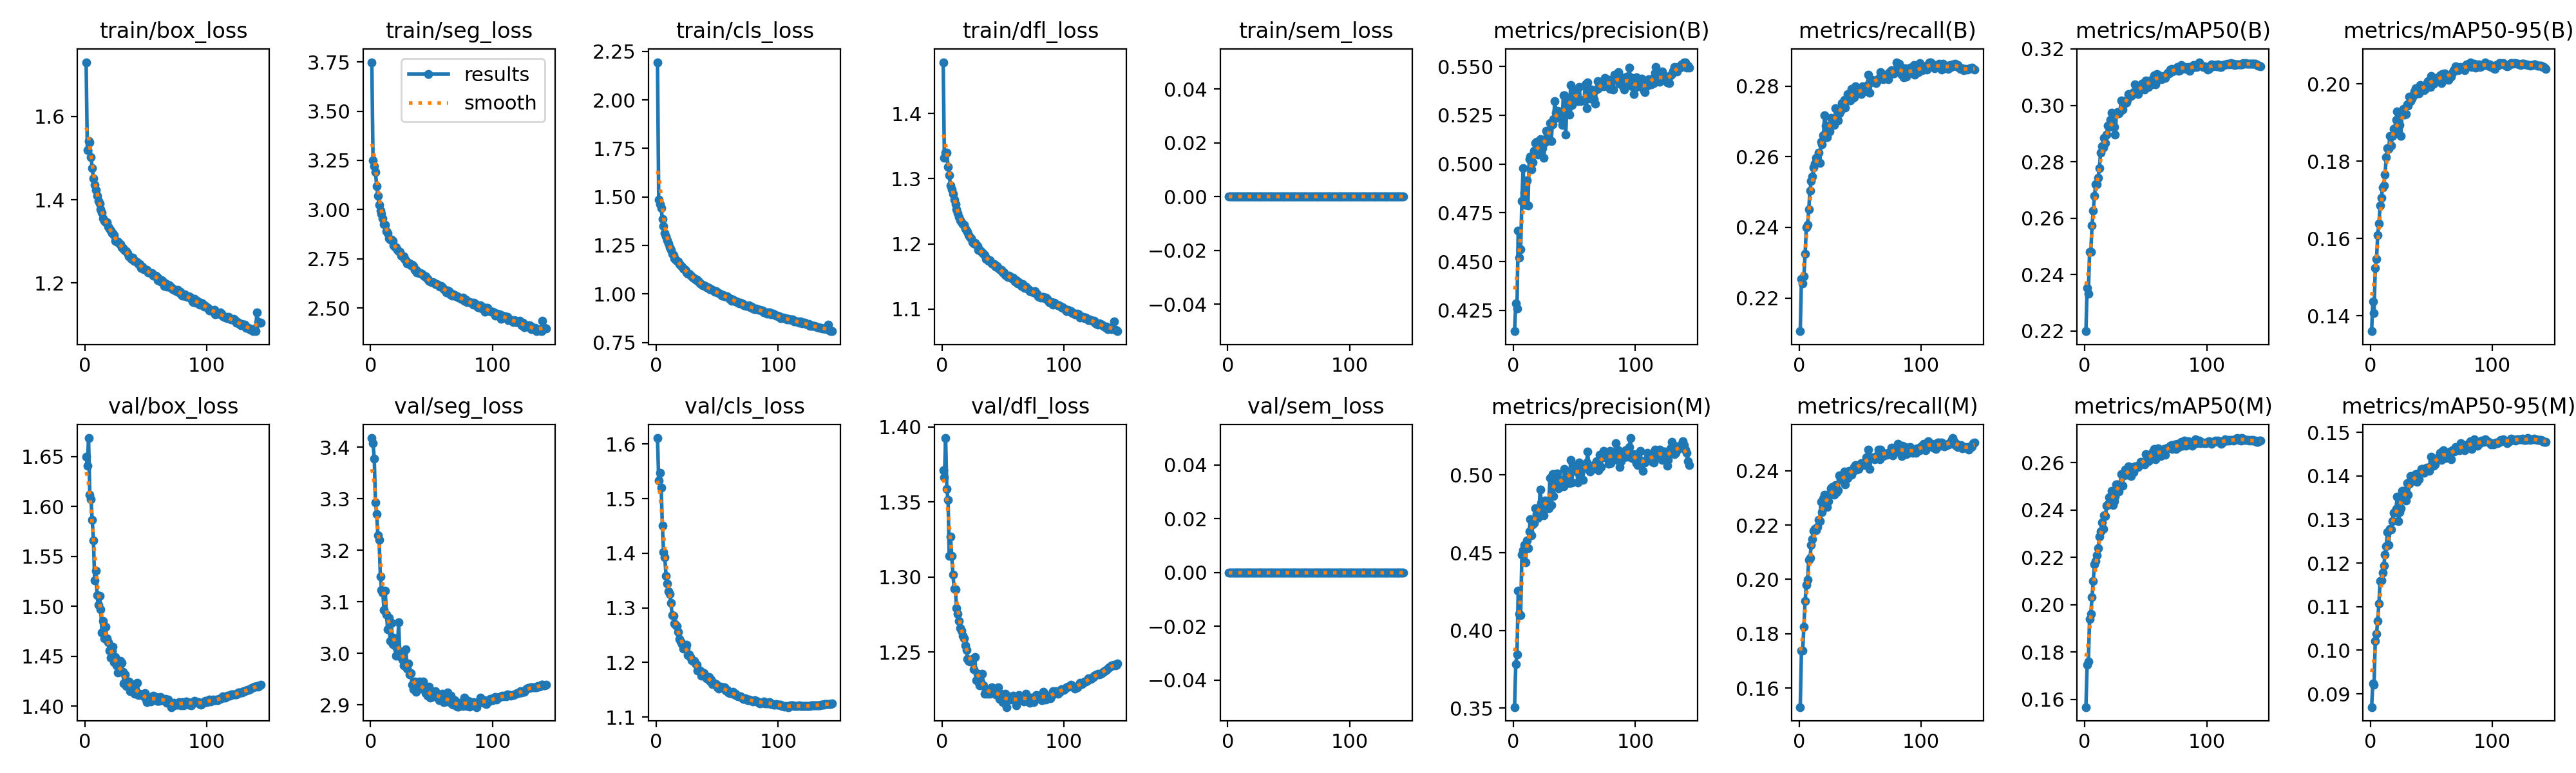
\includegraphics[width=0.78\linewidth]{img/v8s/RESULTS_V8s.png}
    \caption{Результаты обучения сегментатора YOLOv8s-seg}
    \label{fig:8sres}
\end{figure}

По матрице ошибок, видно что модель YOLOv8s-seg, чуть лучше распознает трамвайные пути и рельсы. 59\% для трамвайных путей, 60\% для путей в целом и 51\% для железной дороги как видно из рисунка \ref{fig:8smat}.
\begin{figure}[H]
    \centering
    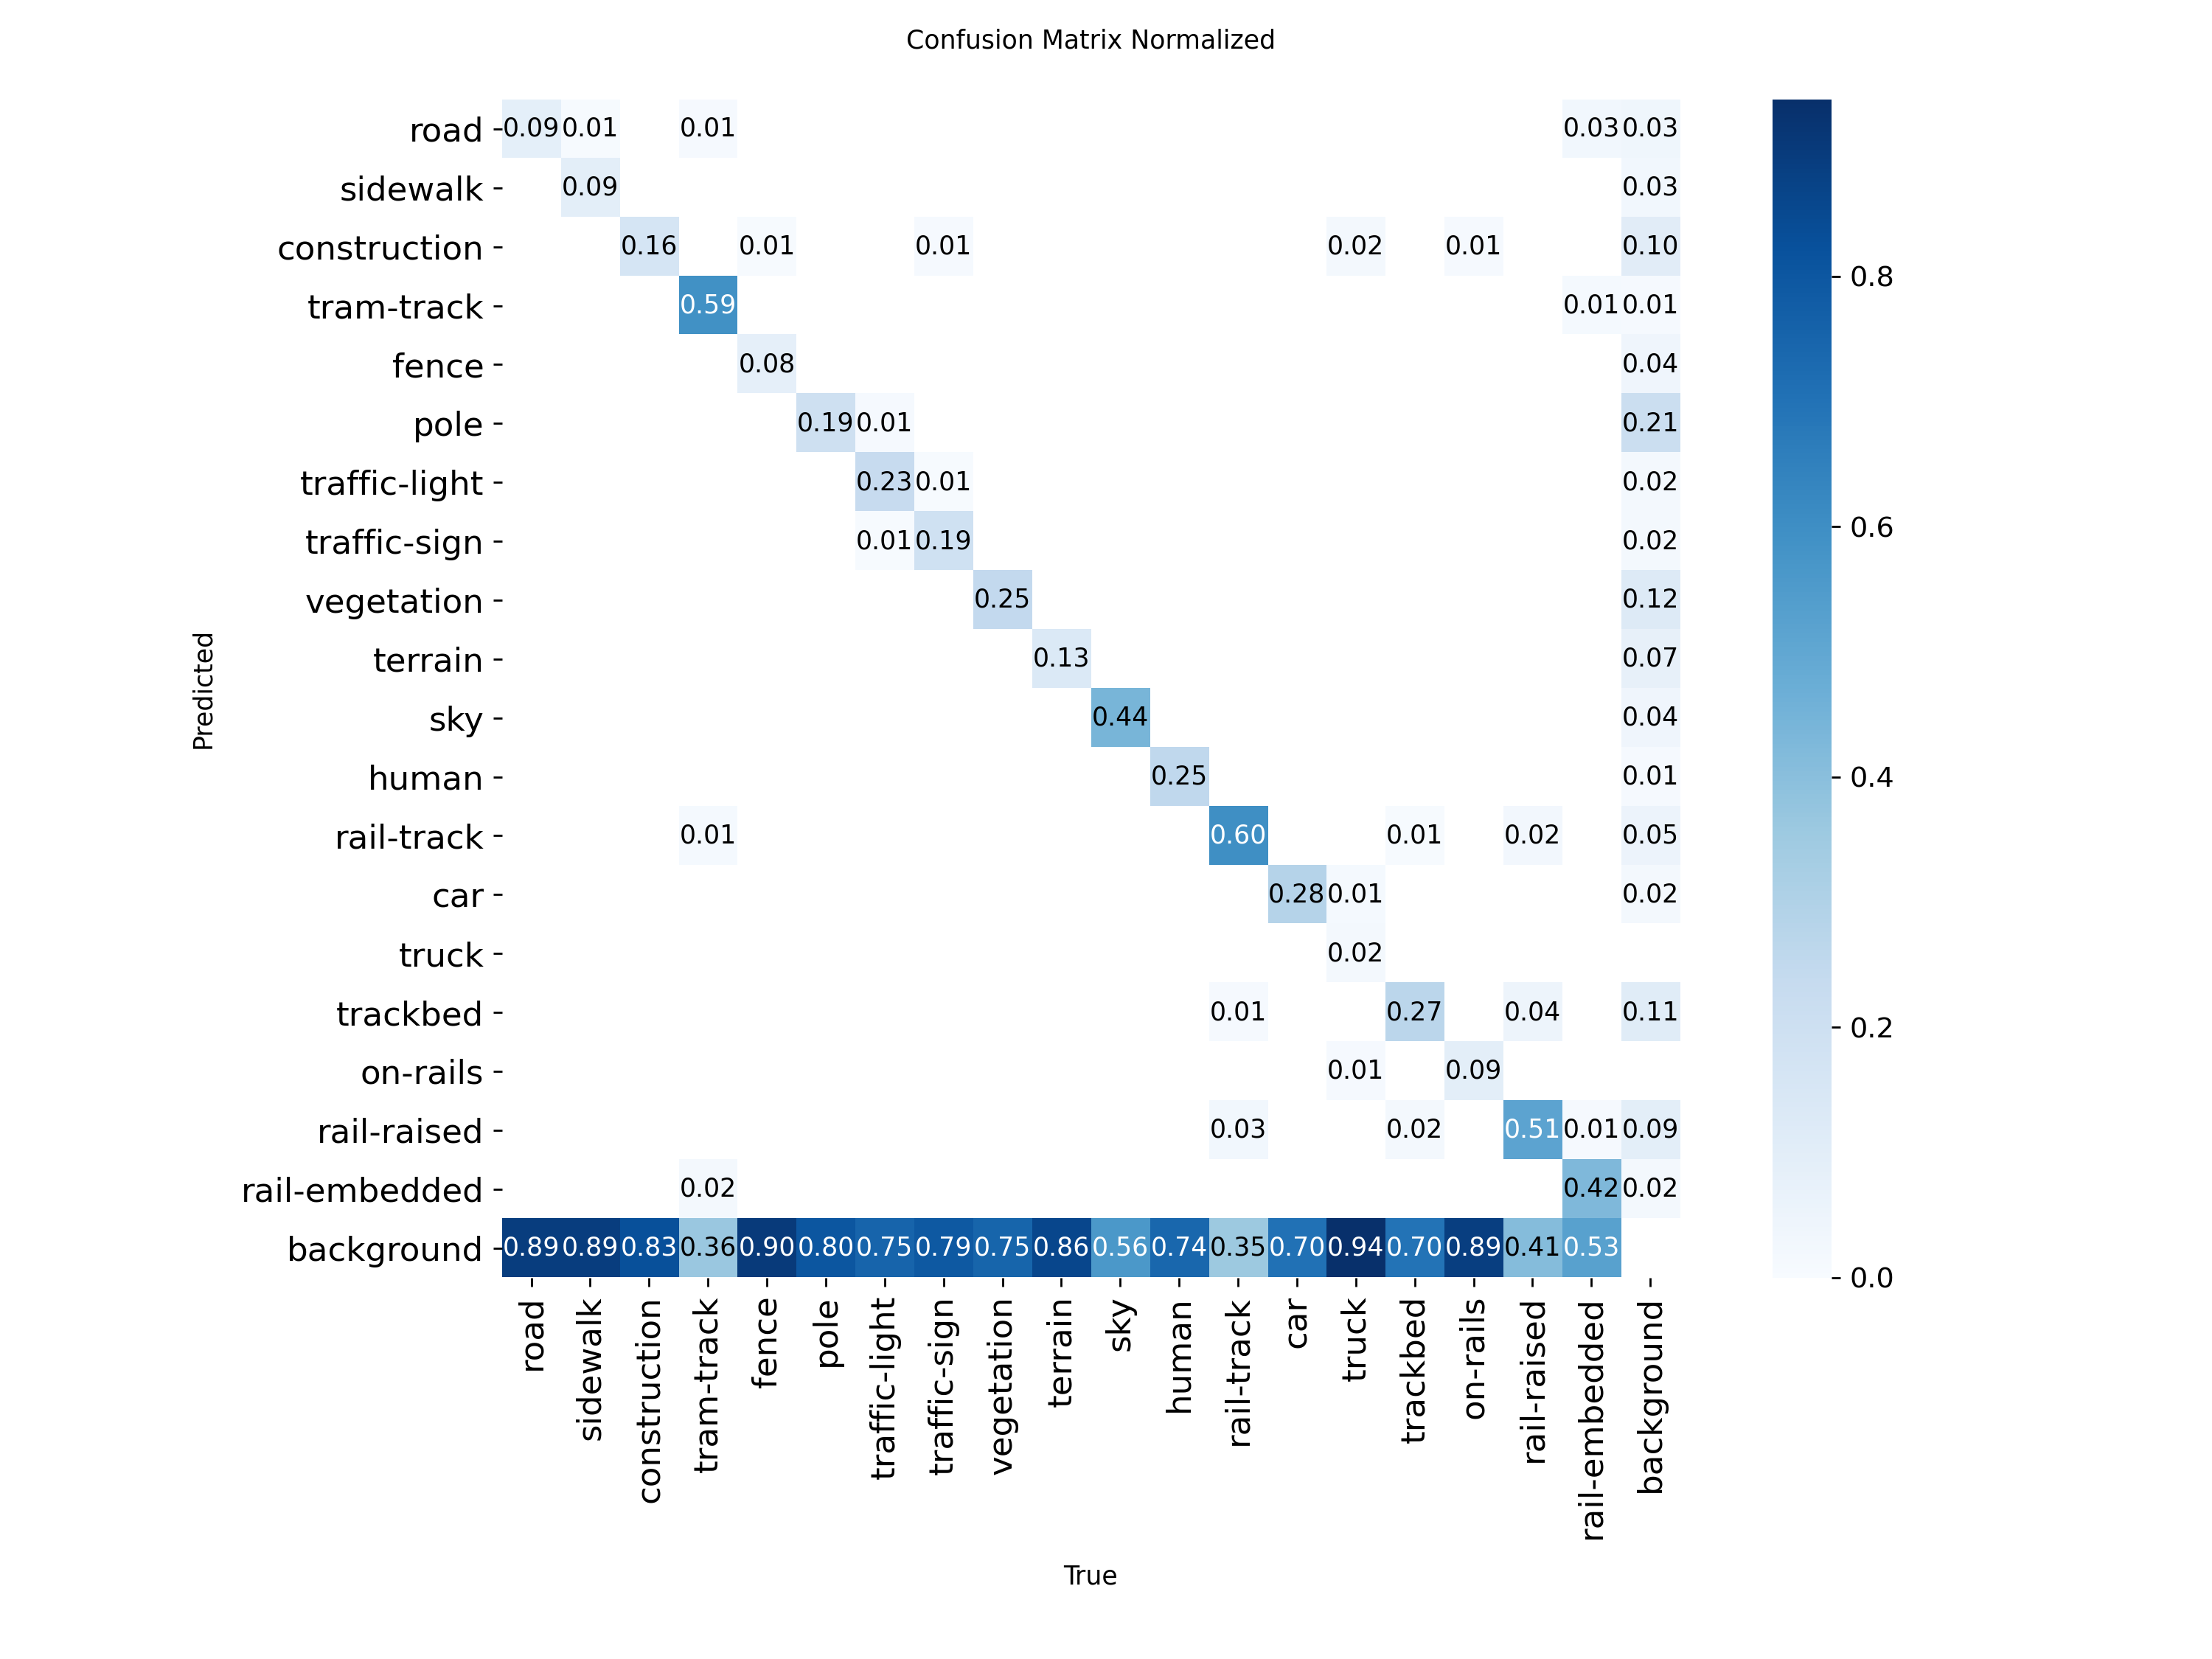
\includegraphics[width=0.58\linewidth]{img/v8s/MATRIX_V8s.png}
    \caption{Матрица ошибок обучения сегментатора YOLOv8s-seg}
    \label{fig:8smat}
\end{figure}


\subsection{Результаты обучения сегментатора YOLOv11s-seg}

Хорошие результаты показала модель YOLOv11s-seg, которая так же обучалась все 150 эпох. Модель является более лучшей версией YOLOv8s-seg, 
скорее всего показатели выше так как точность сегментации выше из-за того что рельсы на изображениях в дальном виде отображаются как несколько пикселей которые YOLOv8s-seg и YOLOv8n-seg игнорировали. 

По графикам обучения, видно что модель еще могла обучатся, так как и на валидации и на обучении наблюдаются признаки недообучения. 
Все графики (кроме графиков метрик точностей) стремятся вниз и не выходят на плато. 

\begin{figure}[H]
    \centering
    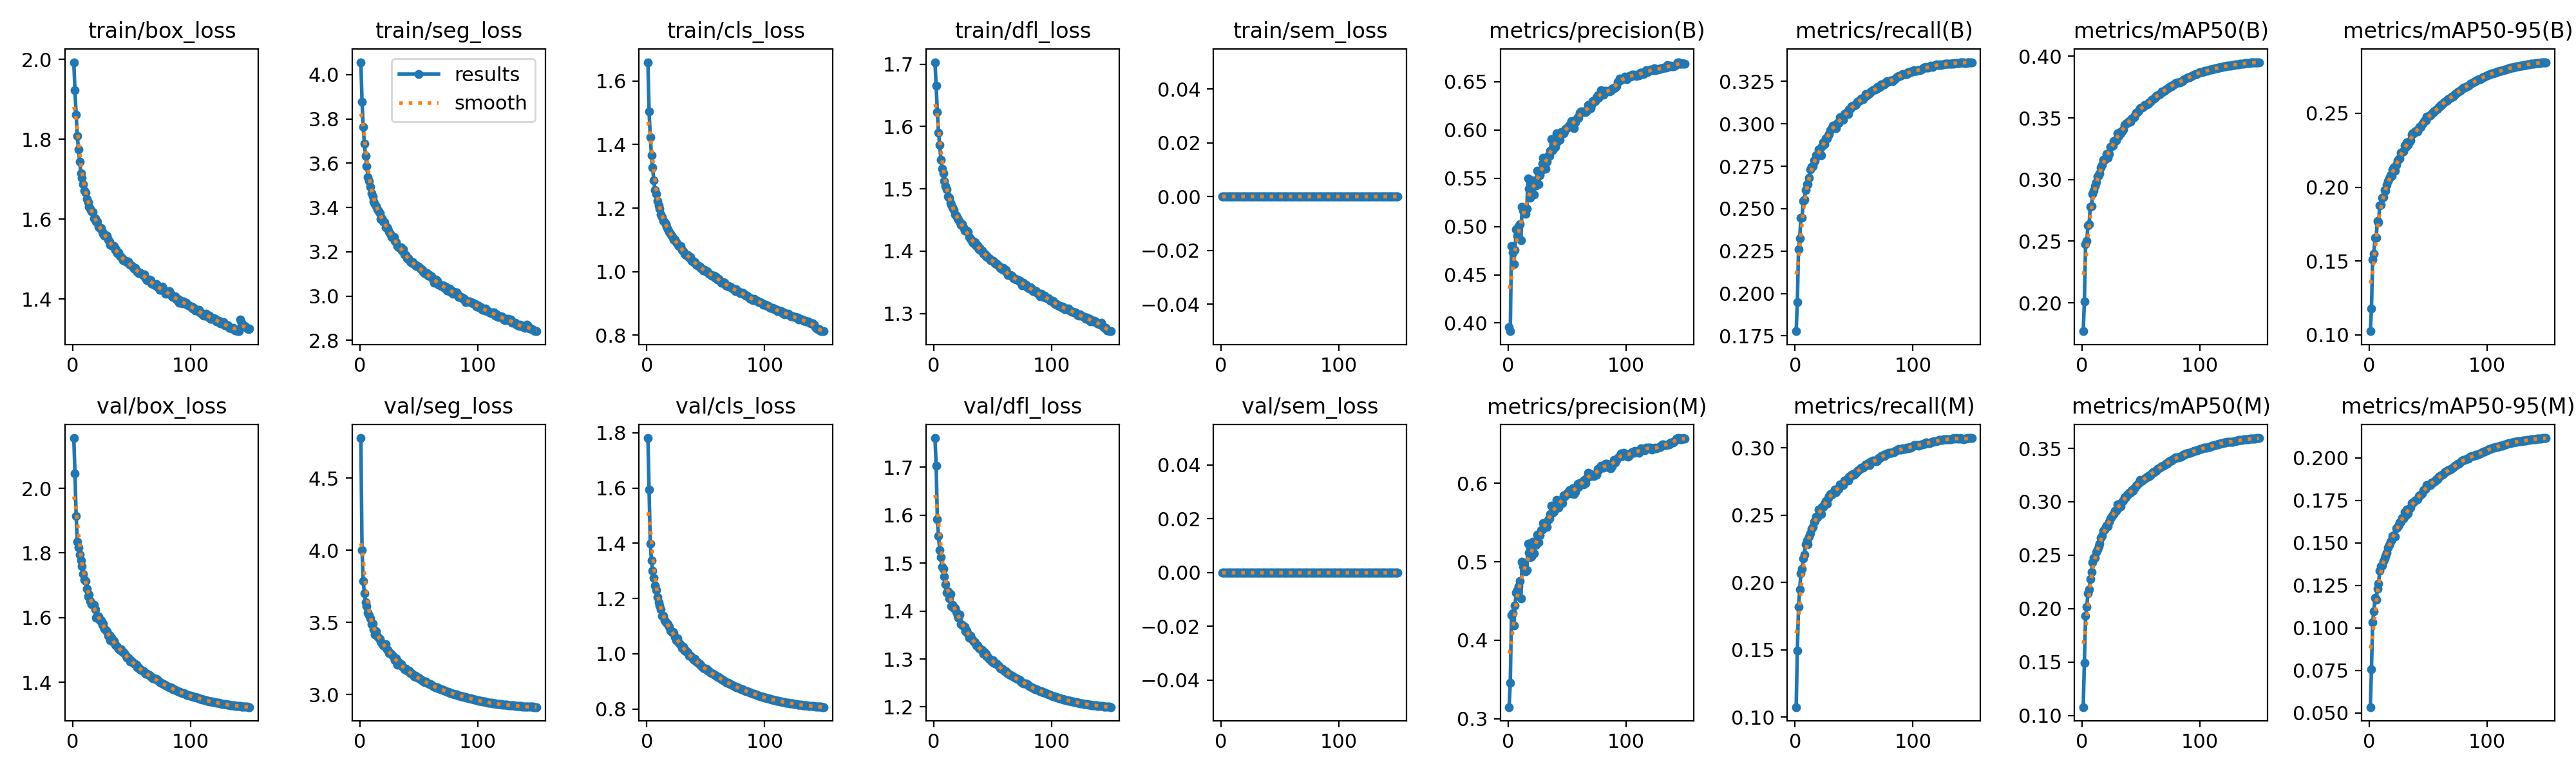
\includegraphics[width=0.78\linewidth]{img/v11s/RESULTS_V11s.png}
    \caption{Результаты обучения сегментатора YOLOv11s-seg}
    \label{fig:11sres}
\end{figure}

По матрице ошибок, YOLOv11s-seg, показала удовлетворительные результаты которые подходят для критерия точности: 71\% для трамвайных путей, 68\% для путей в целом и 65\% для железной дороги (см. рисунок \ref{fig:11smat}).

\begin{figure}[H]
    \centering
    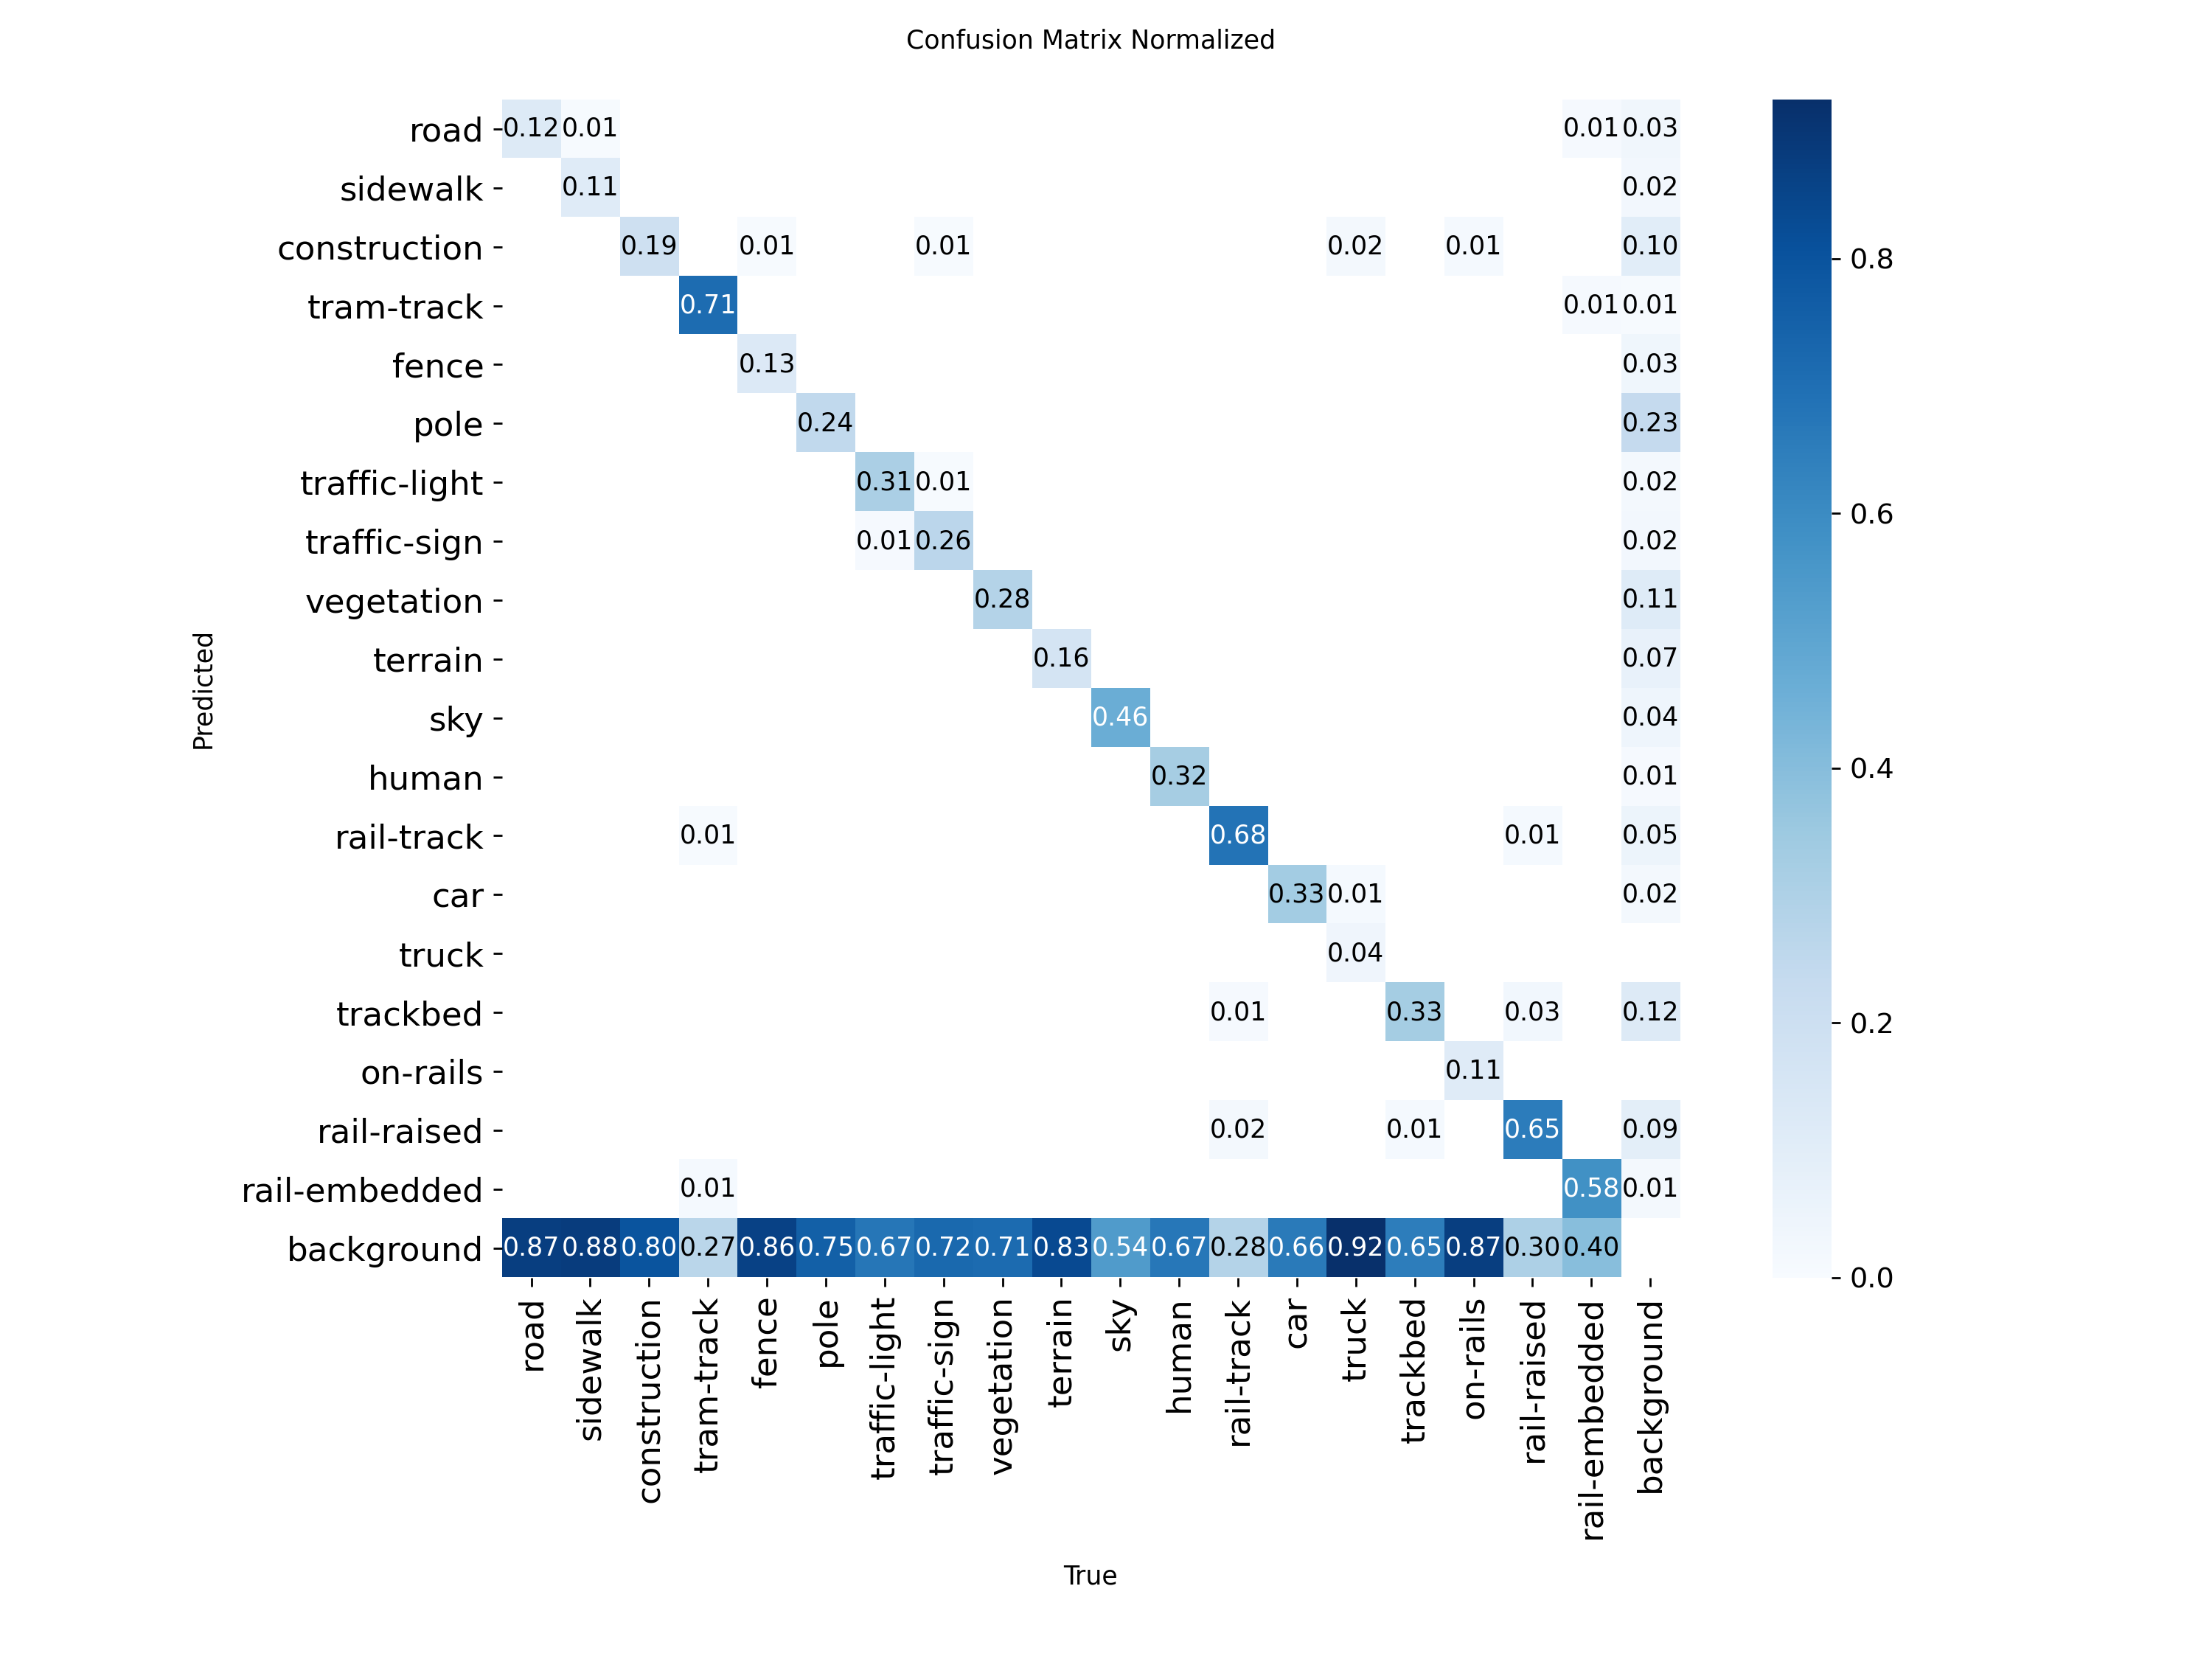
\includegraphics[width=0.58\linewidth]{img/v11s/MATRIX_V11s.png}
    \caption{Матрица ошибок обучения сегментатора YOLOv11s-seg}
    \label{fig:11smat}
\end{figure}


\subsection{Результаты обучения сегментатора YOLO26s-seg}

Модель YOLO26s-seg, обучалась так же все 150 эпох. На графиков так же наблюдается признаки недообучения на валидации.
При этом на обучении наблюдаются резкие скачки на обучении примерно все на 140 эпохи. 
Возможно модели нужно было обучаться дольше, но так же возможно что новая модель действительно не подходит для датасета RailSem19.

\begin{figure}[H]
    \centering
    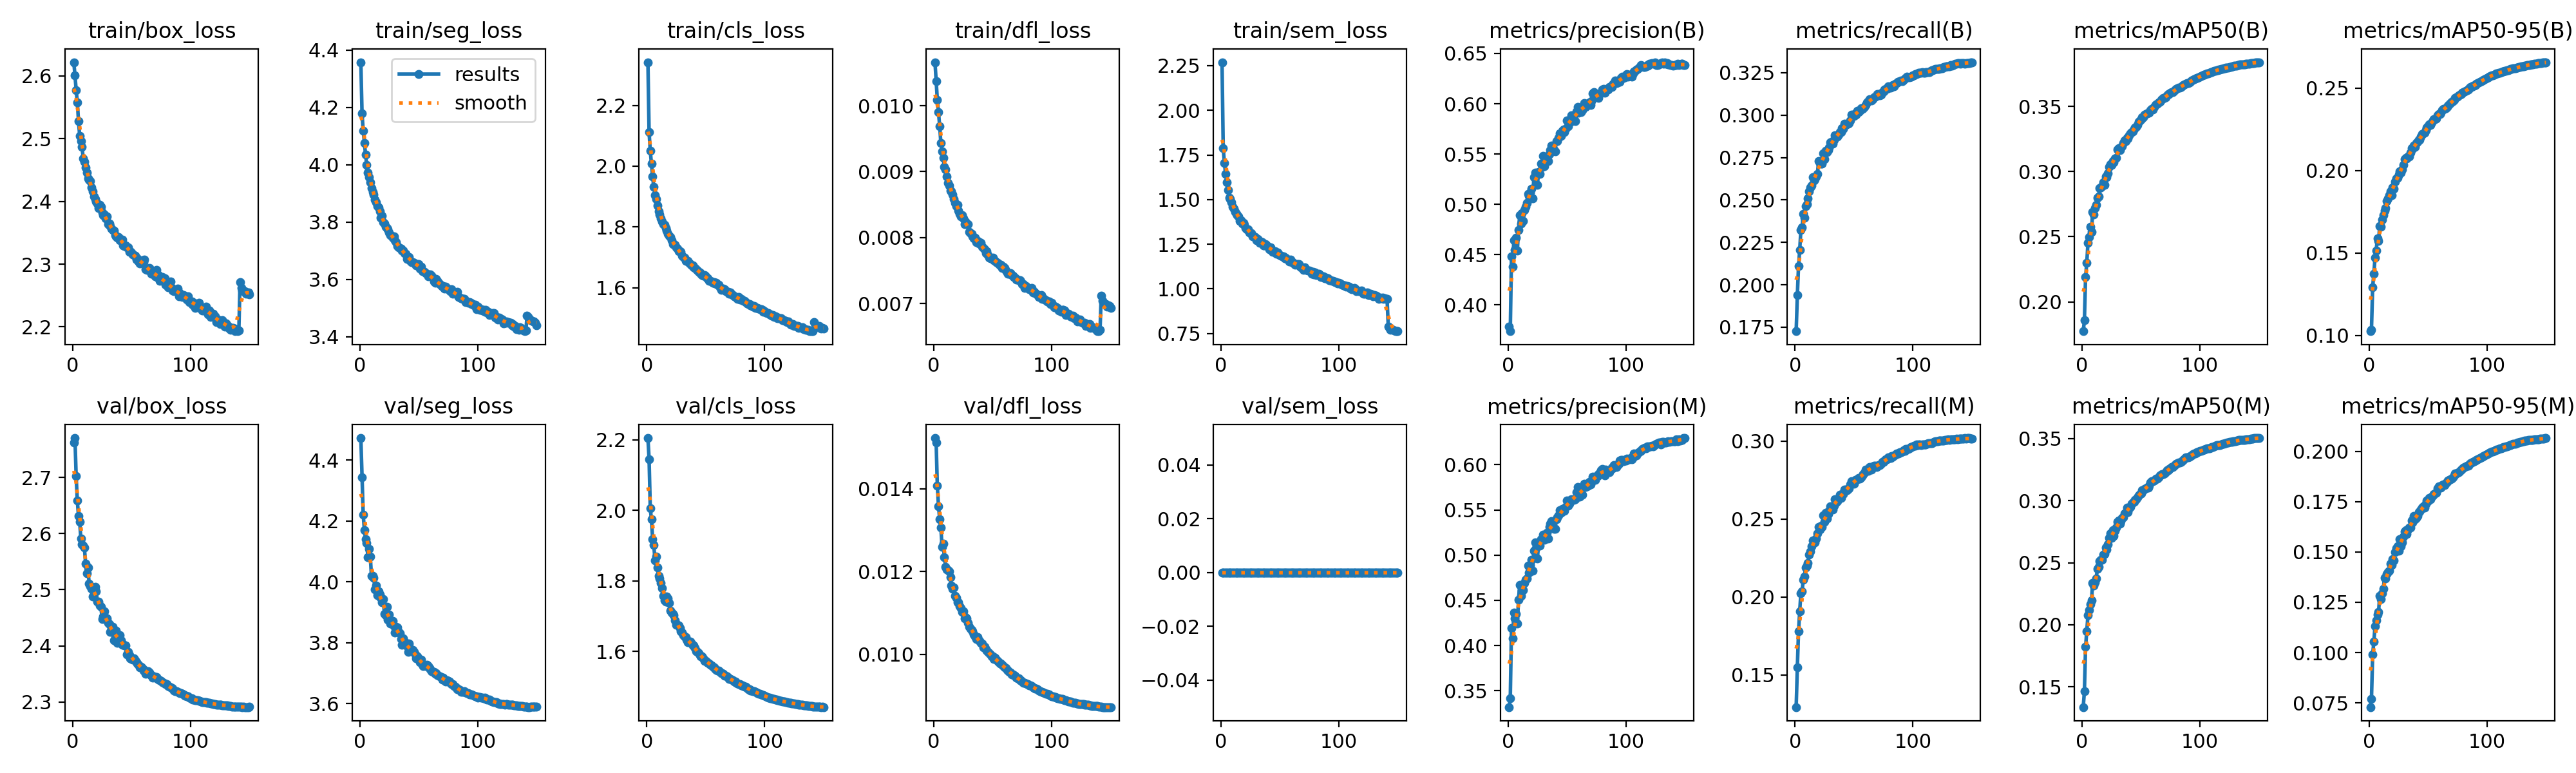
\includegraphics[width=0.78\linewidth]{img/v26s/RESULTS_26s.png}
    \caption{Результаты обучения сегментатора YOLO26s-seg}
    \label{fig:26sres}
\end{figure}

\begin{figure}[H]
    \centering
    \includegraphics[width=0.58\linewidth]{img/v26s/MATRIX_26S.png}
    \caption{Матрица ошибок обучения сегментатора YOLO26s-seg}
    \label{fig:26smat}
\end{figure}

По матрице ошибок результаты хуже чем у YOLOv11s-seg, но лучше чем у YOLOv8s-seg и YOLOv8n-seg: 69\% для трамвайных путей, 63\% для путей в целом и 59\% для железной дороги (см. рисунок \ref{fig:26smat}).

\subsection{Результаты обучения SegFormer B0}

Для обучения сегментатора SegFormer, были найдены оптимальные гиперпараметры находящиеся в открытом доступе из источника \cite{segformer}.

После обучения сегментатора, были получены следующие результаты: 

На рисунке \ref{fig:segloss} представлены значения функции потерь на эпохах обучения SegFormer B0, 
сегментатор обучался 122 эпохи, после чего сработал останов обучения так как значения функции не менялись 15 эпох.

\begin{figure}[H]
    \centering
    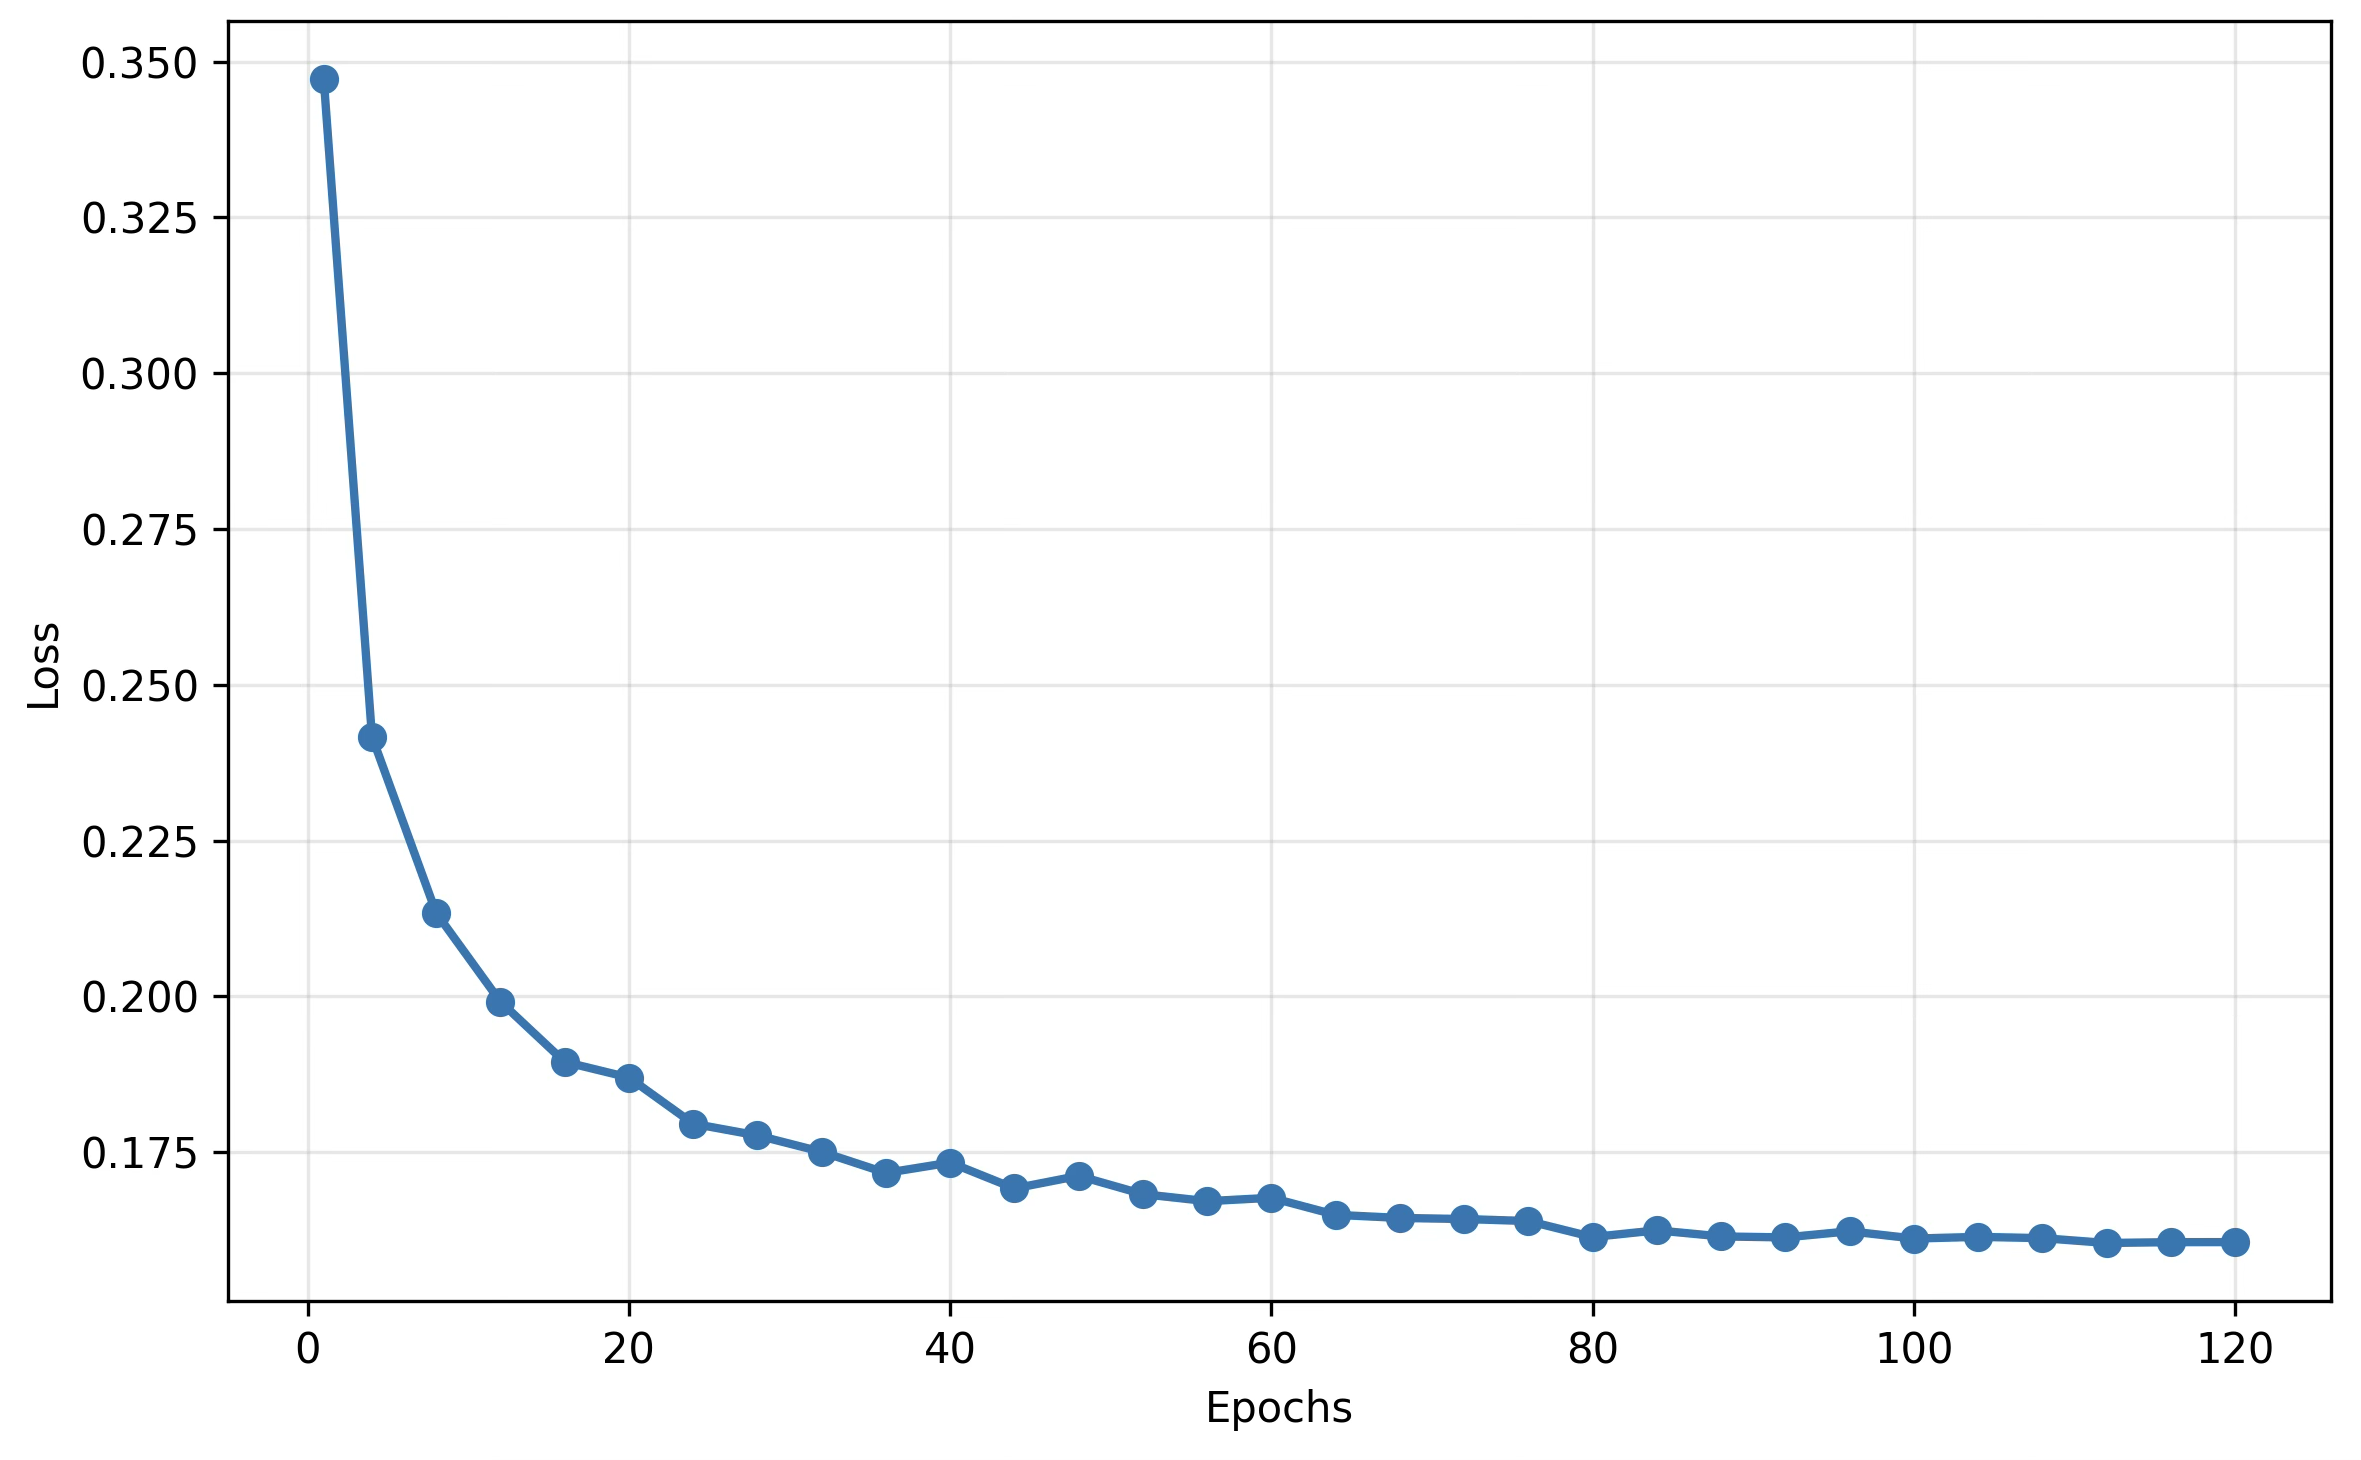
\includegraphics[width=0.78\linewidth]{img/segformer/LOSS.png}
    \caption{Значения функции потерь на эпохах обучения SegFormer B0}
    \label{fig:segloss}
\end{figure}

На рисунке \ref{fig:lrsegformer} представлены значения learning rate на эпохах обучения SegFormer B0:
\begin{figure}[H]
    \centering
    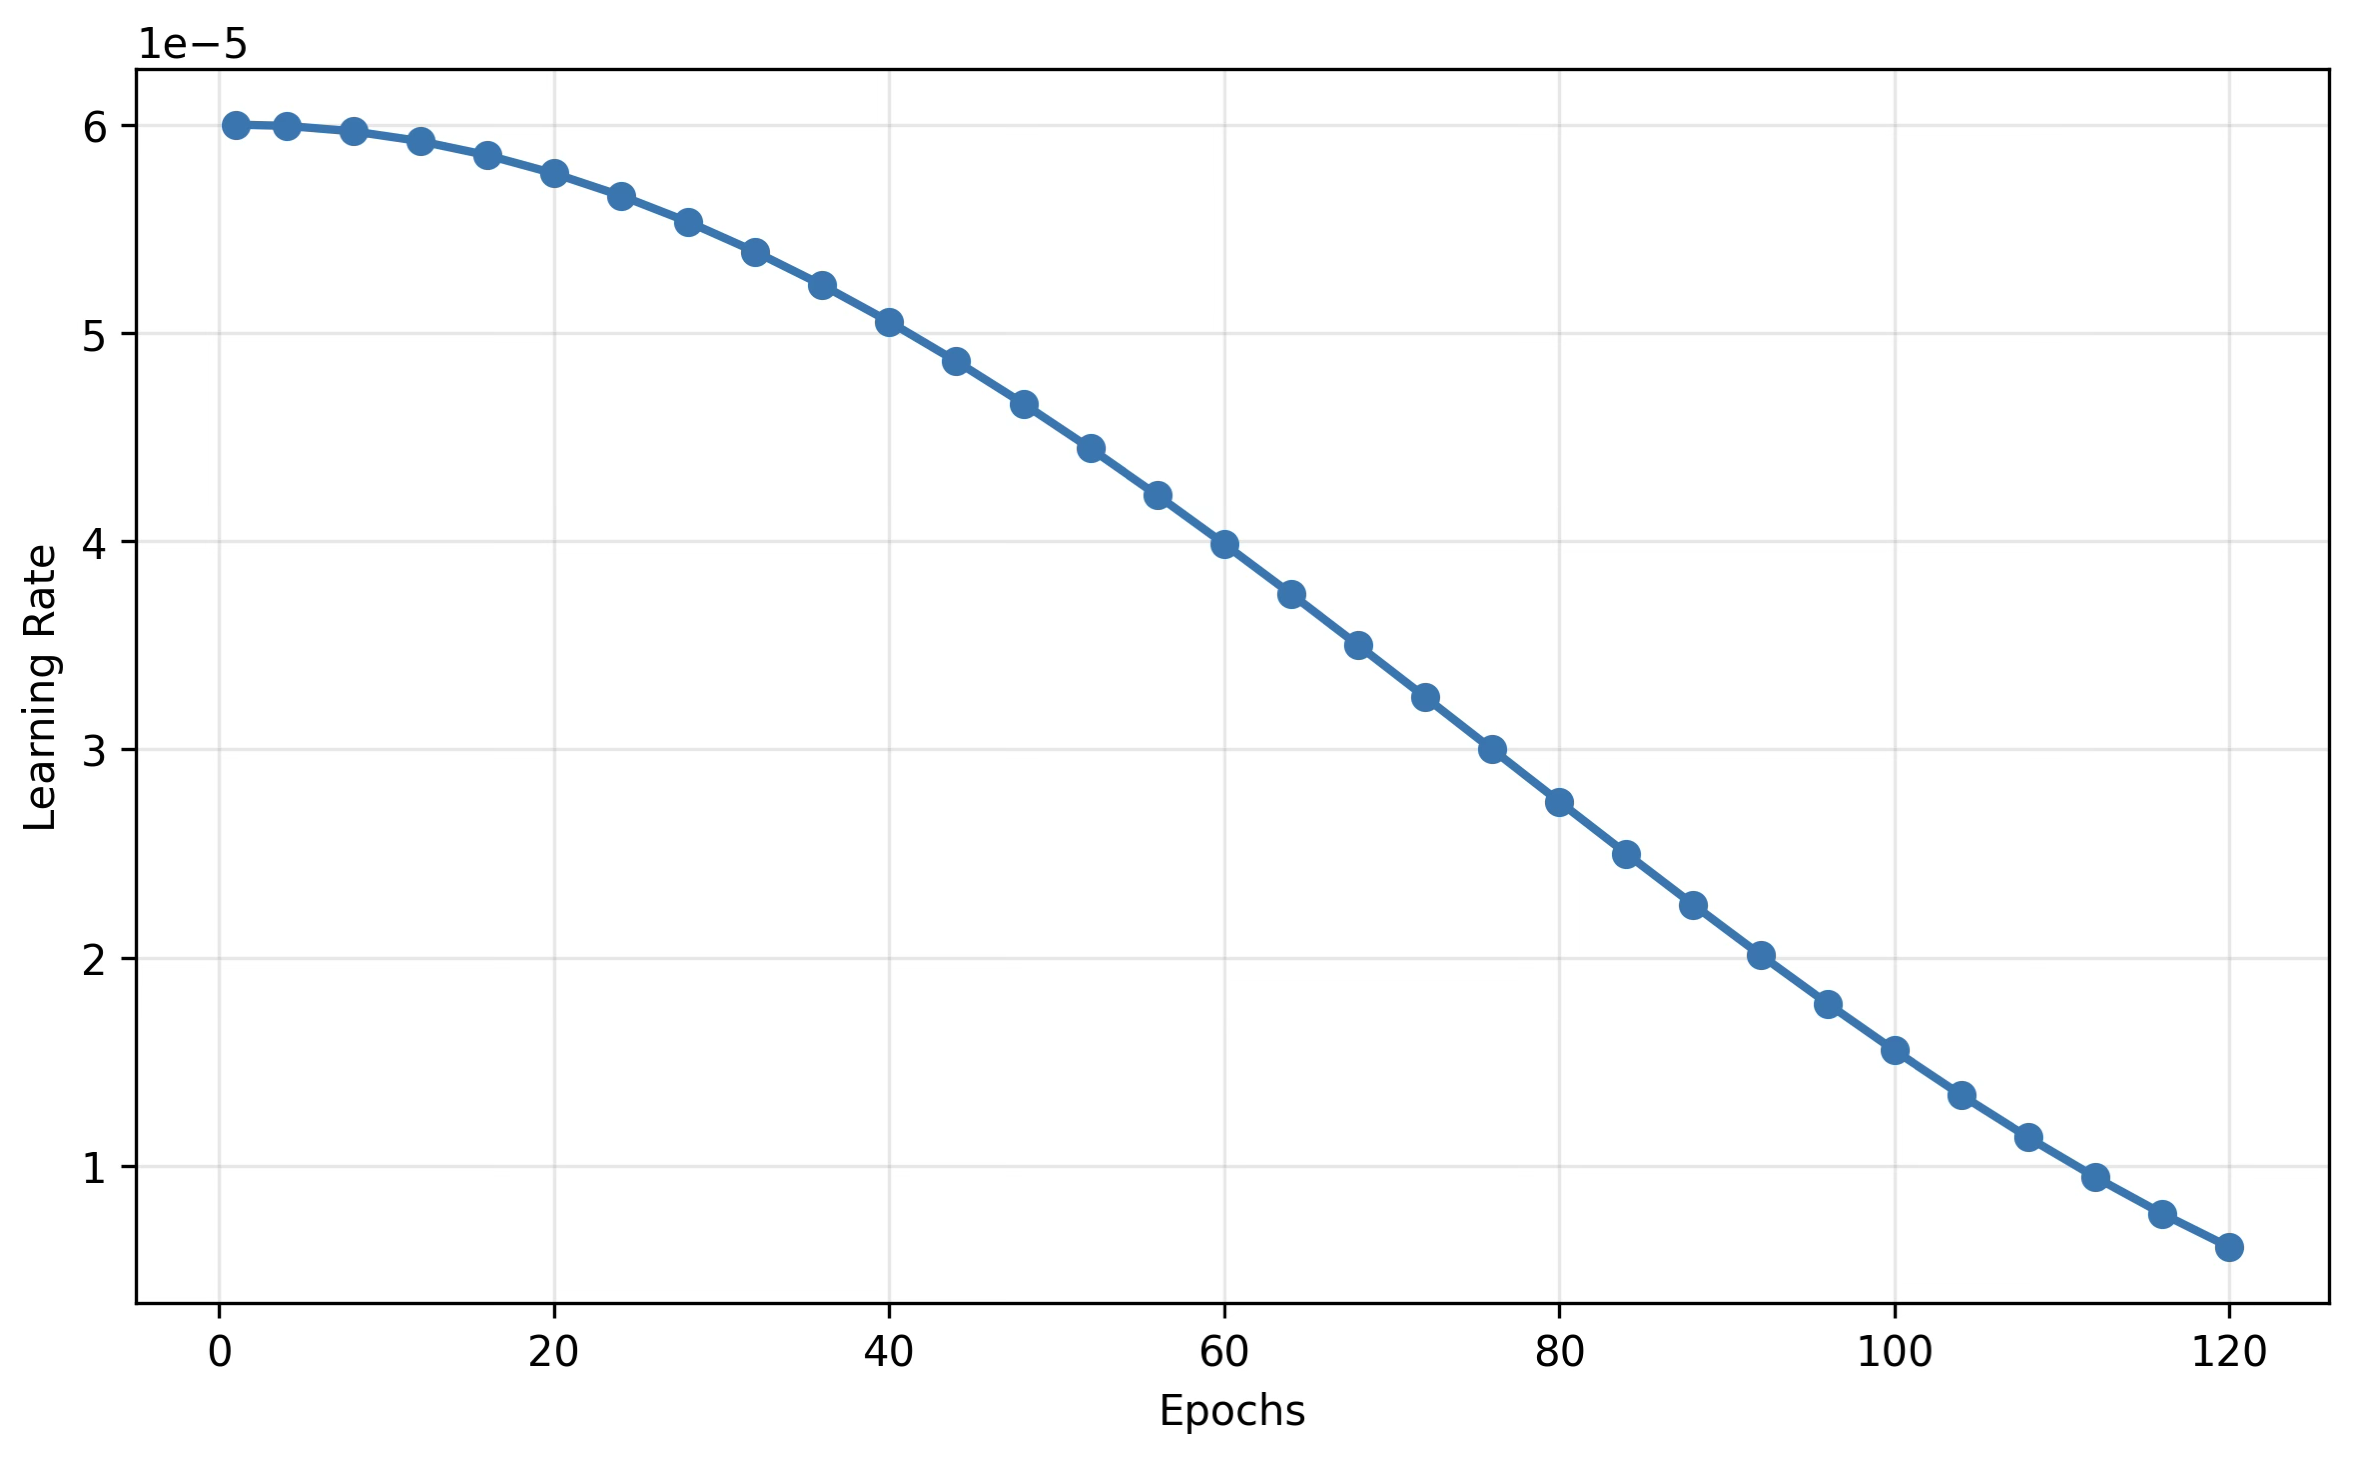
\includegraphics[width=0.78\linewidth]{img/segformer/LR.png}
    \caption{Значения learning rate на эпохах обучения SegFormer B0}
    \label{fig:lrsegformer}
\end{figure}

Как видно, скорость обучения постепенно снижалась до последней эпохи обучения при этом могло бы спускаться дальше но остановилась на эпохе 122.

\subsection{DeepLabV3+ ResNet101}

Обучение сегментатора DeepLabV3+ с энкодером ResNet101, было проведено с помощью библиотеки PyTorch.

Веса модели находились в открытом доступе \cite{deeplab_railsem}, что не потребывало дополнительного обучения модели.


\newpage
\section{Анализ результатов}
Исходя из результатов быстрого подбора гиперпараметров и обучения сегментаторов
был сделан следующий вывод:

\begin{itemize}
    \item \textcolor{red}{DeepLabV3+ с энкодером ResNet101} - оказался слишком медленным и не точным для сегментации трамвайных путей;
    \item \textcolor{orange}{SegFormer B0} - оказался не точным для сегментации и слишком тяжелым для обучения, возможно модели B3, B5, были более точными но, эти модели не преспасоблены на работу в реальном времени;
    \item \textcolor{orange}{YOLOv8n-seg} - оказался самой быстрой моделью однако показал плохие результаты на валидации и не смог пройти критерий точности;
    \item \textcolor{orange}{YOLOv8s-seg} - точность оказалась лучше чем у YOLOv8n-seg, но так же не смогла пройти критерий точности, при этом были явные признаки переобучеиня;
    \item \textcolor{green}{YOLOv11s-seg} - показала лучшие результаты как по скорости так и по точности распознавания, модель явно стоит дообучать;
    \item \textcolor{blue}{YOLO26s-seg} - показала результаты хуже чем у YOLOv11s-seg, но лучше чем у других моделей, однако модель либо не подходит для выбранного датасета, либо для новой модели нужно искать новые гиперпараметры. Однако как видно из результатов, модели YOLOv11s-seg вполне хватает для решения поставленной задачию.
\end{itemize}

Ниже на рисунках \ref{fig:segformerres} - \ref{fig:26sresseg}, представлены результаты сегментации а так же скорость их инференса: 

\begin{figure}[H]
    \centering
    
\includegraphics[width=0.78\linewidth]{img/res/SEGFORMER.png}
    \caption{Результаты сегментации SegFormer}
    \label{fig:segformerres}
\end{figure}

Результат: 
\begin{itemize}
    \item Средняя скорость: 32 FPS
    \item Средняя точность: 64\%
\end{itemize}

\begin{figure}[H]
    \centering
    
\includegraphics[width=0.78\linewidth]{img/res/DEEPLAB.png}
    \caption{Результаты сегментации DeepLabV3+}
    \label{fig:deeplabres}
\end{figure}

Результат: 
\begin{itemize}
    \item Средняя скорость: $\leq 1$ FPS
    \item Средняя точность: 41\%
\end{itemize}

\begin{figure}[H]
    \centering
    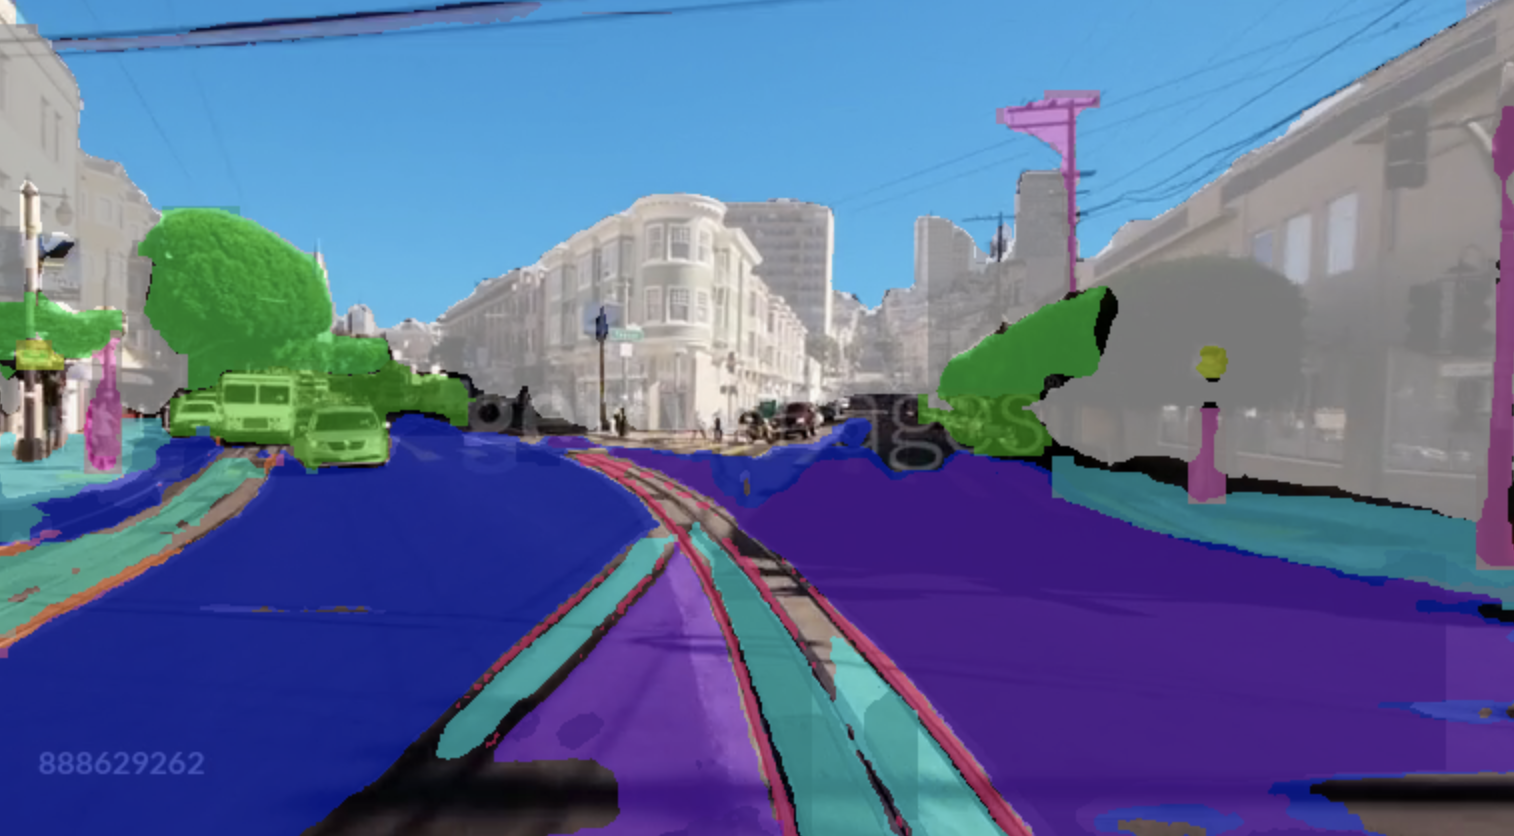
\includegraphics[width=0.78\linewidth]{img/res/8N.png}
    \caption{Результаты сегментации YOLOv8n-seg}
    \label{fig:8nresseg}
\end{figure}

Результат: 
\begin{itemize}
    \item Средняя скорость: 34 FPS
    \item Средняя точность: 55\%
\end{itemize}

\begin{figure}[H]
    \centering
    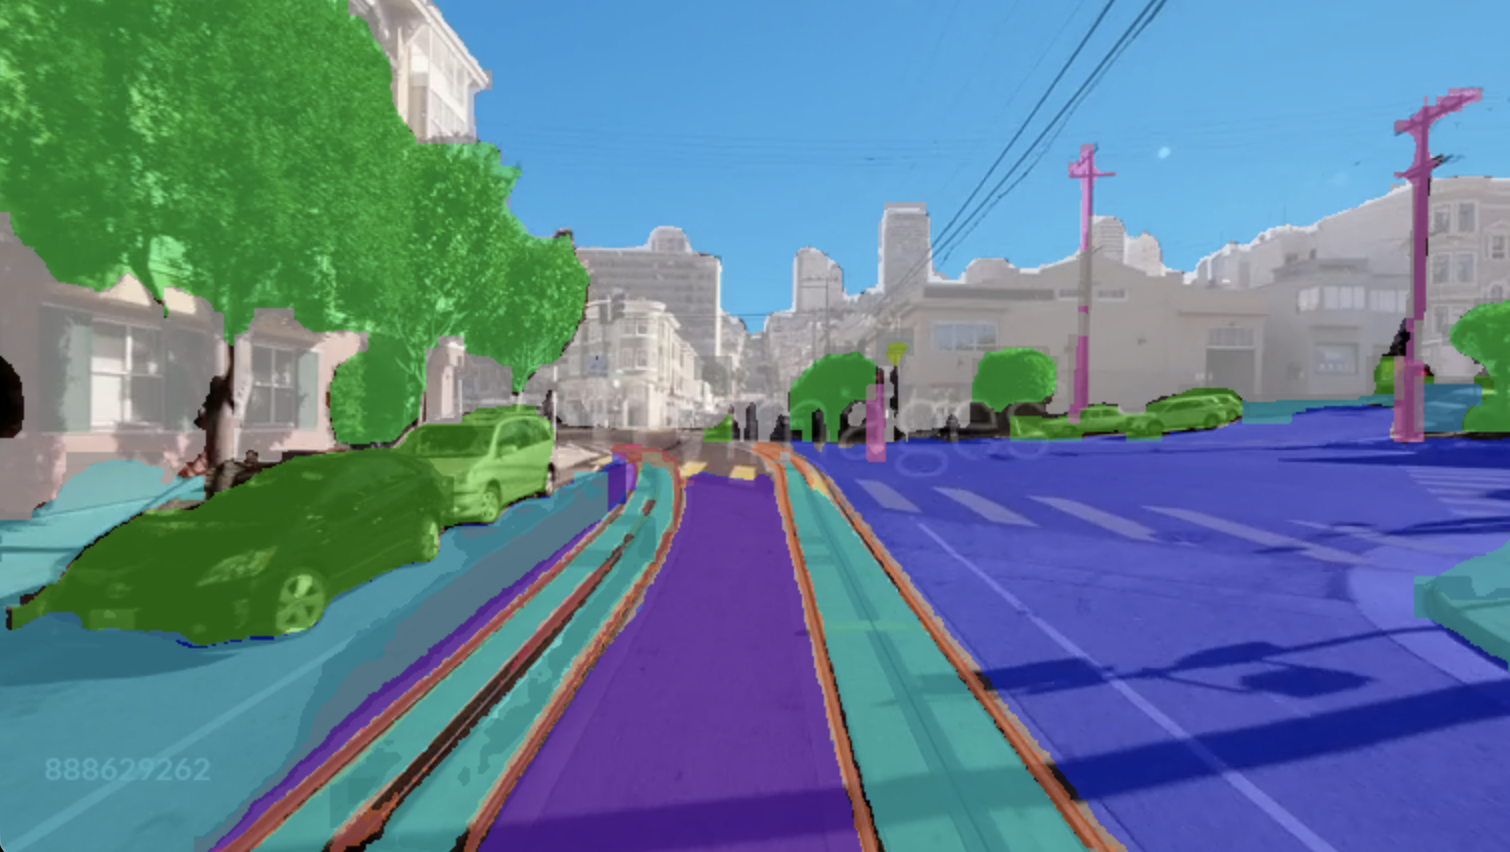
\includegraphics[width=0.78\linewidth]{img/res/8S.png}
    \caption{Результаты сегментации YOLOv8s-seg}
    \label{fig:8sresseg}
\end{figure}

Результат: 
\begin{itemize}
    \item Средняя скорость: 30 FPS
    \item Средняя точность: 62\%
\end{itemize}

\begin{figure}[H]
    \centering
    
\includegraphics[width=0.78\linewidth]{img/res/11.png}
    \caption{Результаты сегментации YOLOv11s-seg}
    \label{fig:11sresseg}
\end{figure}

Результат: 
\begin{itemize}
    \item Средняя скорость: 31 FPS
    \item Средняя точность: 71\%
\end{itemize}

\begin{figure}[H]
    \centering
    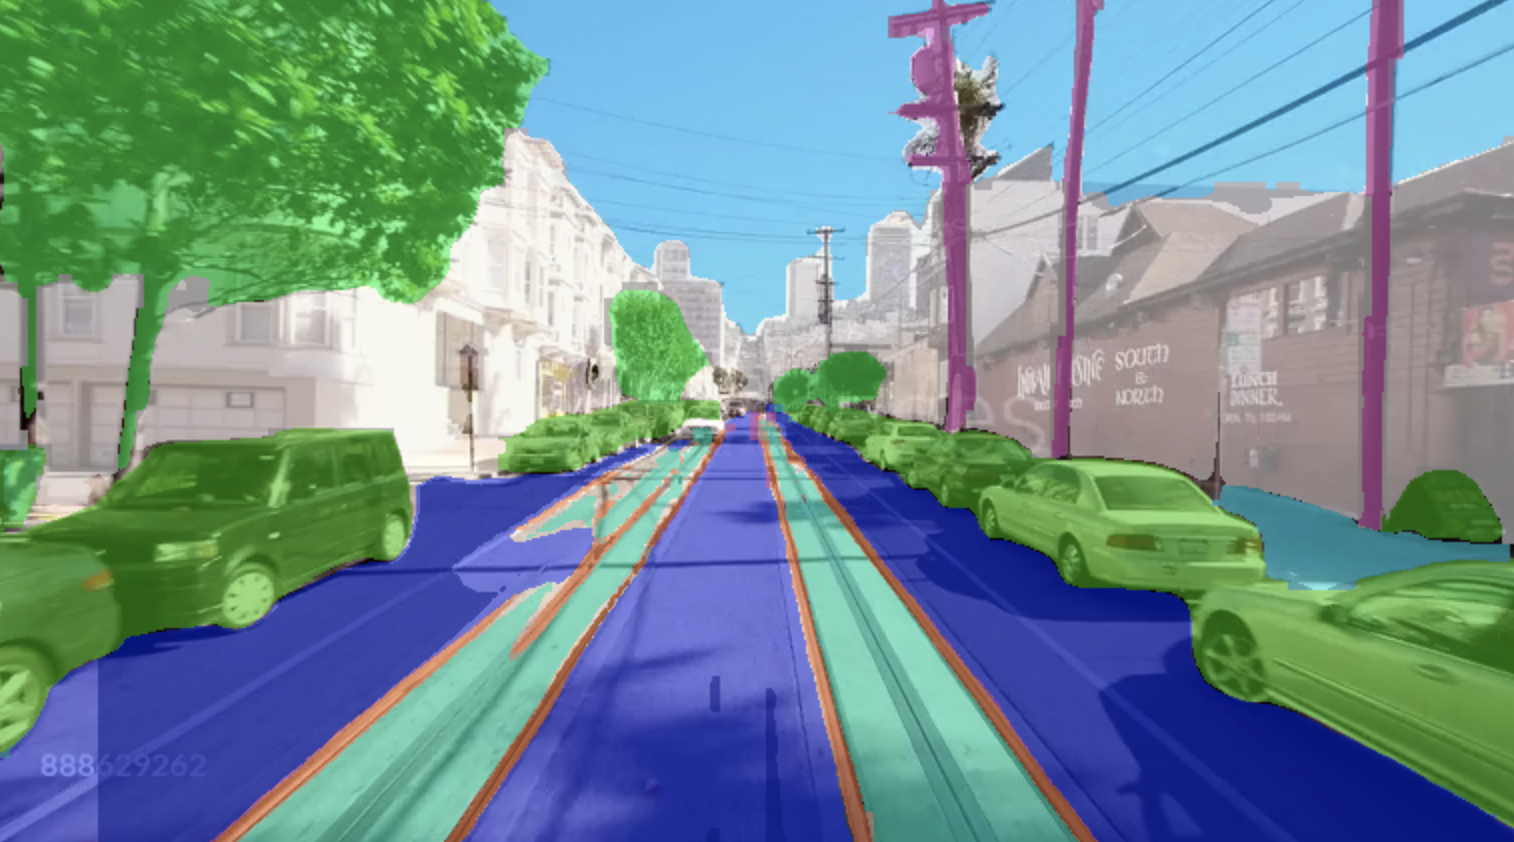
\includegraphics[width=0.78\linewidth]{img/res/26.png}
    \caption{Результаты сегментации YOLO26s-seg}
    \label{fig:26sresseg}
\end{figure}

Результат: 
\begin{itemize}
    \item Средняя скорость: 32 FPS
    \item Средняя точность: 69\%
\end{itemize}

\newpage
\section*{Заключение}
\addcontentsline{toc}{section}{Заключение}
Выбранная модель YOLOv11s-seg, будет использоваться для дальнейшего поиска оптимальных гиперпараметров, с помощью библиотеки Optune, 
которая ищет оптимальные гиперпараметры более точно, но так же является более тяжелой для подбора. 

Так же в последствии будет использоваться кросс-валидация с методом leave one out и пятью блоками (Fold), для более точной оценки модели.

Далее разрабатывается алгоритм выделения зоны интереса RoI, дорисовкой полигонов вокруг сегментированных рельс, и реализация инференса модели YOLOv8s для детекции посторонних объектов в режиме реального времени.

\newpage
\addcontentsline{toc}{section}{Список литературы}
\begin{thebibliography}{99}
    \bibitem{skobtsov}
    Скобцов Ю.\,А., Сперанский Д.\,В. Эволюционные вычисления: Учебное пособие. – М.: Национальный Открытый Университет «ИНТУИТ», 2012. – 331\,с., ил. – (Серия «Основы информационных технологий»).

    \bibitem{aliev}
    Алиев М.\,В., Бербенцев Д.\,А., Немыкин В.\,О., Алиева С.\,М. Алгоритмы распознавания объектов в видеопотоке и определение свойств их взаимного расположения // Вестник Адыгейского государственного университета. Сер. Естественно-математические и технические науки. – 2024. – №\,2(341). – С.\,27–34. DOI: 10.53598/2410-3225-2024-2-341-27-34.

    \bibitem{zotov}
    Зотов С.\,С., Яковлев А.\,А., Колчищев Д.\,А. Обнаружение объектов в реальном времени с помощью алгоритмов распознавания YOLO // Синергия наук. – 2018. – №\,23. – С.\,1245–1261.

    \bibitem{chochia}
    Чочиа П.\,А. Сегментация изображений на основе анализа расстояний в пространстве признаков // Информационные процессы. – 2020. – №\,6. – С.\,97–110.

    \bibitem{zhang}
    Zhang H., Ullah N., Sharnah A. CA-SegFormer: An improved coordinate attention-enhanced model for crack segmentation in concrete structures // Case Studies in Construction Materials. – 2025. – Vol.\,23.

    \bibitem{yanyan}
    Yanyan Z., Zhiliang S. Adioc loss: An Auxiliary descent IoC loss function // Engineering Applications of Artificial Intelligence. – 2022. – №\,105453. – С.\,117–133. DOI: https://doi.org/10.1016/j.engappai.2022.105453.

    \bibitem{yolov8doc}
    YOLOv8 Documentation [Электронный ресурс] // Ultralytics. – Доступ: \url{https://docs.ultralytics.com/ru/models/yolov8/} (дата обращения: 07.02.2026).

    \bibitem{yolov5doc}
    YOLOv5 Documentation [Электронный ресурс] // Ultralytics. – Доступ: \url{https://docs.ultralytics.com/ru/models/yolov5/} (дата обращения: 07.02.2026).

    \bibitem{xie_segformer}
    Xie E., Wang W., Yu Z., Anandkumar A., Alvarez J.\,M., Luo P. SegFormer: Simple and Efficient Design for Semantic Segmentation with Transformers // arXiv [cs.CV]. – 2021. – 28 Oct.

    \bibitem{segformer}
    RailSafeNet. train\_SegFormer.py [Электронный ресурс] // GitHub. – Доступ: \url{https://github.com/oValach/RailSafeNet/blob/main/train_SegFormer.py} (дата обращения: 14.03.2026).

    \bibitem{moroz}
    Мороз Е.\,С., Пикалёв Я.\,С. Анализ SOTA-архитектур для семантической аугментации // Информационные технологии и системы. – 2025. – №\,4. – С.\,39–60. DOI: 10.24412/2413-7383-2025-4-39-60-70.

    \bibitem{xie_mit}
    Xie E., Wang W., Yu Z., Anandkumar A., Alvarez J.\,M., Luo P. Details of MiT Series // arXiv [cs.CV]. – 2021. – (Supplementary material).

    \bibitem{deeplab_railsem}
    DeepLabV3Plus-RailSem19 [Электронный ресурс] // GitHub. – Доступ: \url{https://github.com/pideyi1025/DeepLabV3Plus-RailSem19/tree/main} (дата обращения: 14.03.2026).

    \bibitem{springer}
    Springer Link. Статья по компьютерному зрению [Электронный ресурс] // Springer. – Доступ: \url{https://link.springer.com/article/10.1007/s11554-023-01380-x} (дата обращения: 14.03.2026).

    \bibitem{ultralytics_segment}
    Instance Segmentation. Val [Электронный ресурс] // Ultralytics. – Доступ: \url{https://docs.ultralytics.com/ru/tasks/segment/#val} (дата обращения: 14.03.2026).

    \bibitem{ultralytics_yolov8}
    YOLOv8. Key Features [Электронный ресурс] // Ultralytics. – Доступ: \url{https://docs.ultralytics.com/ru/models/yolov8/#key-features-of-yolov8} (дата обращения: 14.03.2026).

    \bibitem{ultralytics_yolov11}
    YOLOv11. Key Features [Электронный ресурс] // Ultralytics. – Доступ: \url{https://docs.ultralytics.com/ru/models/yolov11/#key-features-of-yolov11} (дата обращения: 14.03.2026).

    \bibitem{ultralytics_yolo26}
    YOLO26 Documentation [Электронный ресурс] // Ultralytics. – Доступ: \url{https://docs.ultralytics.com/ru/models/yolo26/} (дата обращения: 14.03.2026).

    \bibitem{ultralytics_tune}
    Hyperparameter Tuning [Электронный ресурс] // Ultralytics. – Доступ: \url{https://docs.ultralytics.com/guides/hyperparameter-tuning/} (дата обращения: 14.03.2026).
\end{thebibliography}

\end{document}  